\documentclass[10pt]{beamer}\usepackage[]{graphicx}\usepackage[]{color}
%% maxwidth is the original width if it is less than linewidth
%% otherwise use linewidth (to make sure the graphics do not exceed the margin)
\makeatletter
\def\maxwidth{ %
  \ifdim\Gin@nat@width>\linewidth
    \linewidth
  \else
    \Gin@nat@width
  \fi
}
\makeatother

\definecolor{fgcolor}{rgb}{0.345, 0.345, 0.345}
\newcommand{\hlnum}[1]{\textcolor[rgb]{0.686,0.059,0.569}{#1}}%
\newcommand{\hlstr}[1]{\textcolor[rgb]{0.192,0.494,0.8}{#1}}%
\newcommand{\hlcom}[1]{\textcolor[rgb]{0.678,0.584,0.686}{\textit{#1}}}%
\newcommand{\hlopt}[1]{\textcolor[rgb]{0,0,0}{#1}}%
\newcommand{\hlstd}[1]{\textcolor[rgb]{0.345,0.345,0.345}{#1}}%
\newcommand{\hlkwa}[1]{\textcolor[rgb]{0.161,0.373,0.58}{\textbf{#1}}}%
\newcommand{\hlkwb}[1]{\textcolor[rgb]{0.69,0.353,0.396}{#1}}%
\newcommand{\hlkwc}[1]{\textcolor[rgb]{0.333,0.667,0.333}{#1}}%
\newcommand{\hlkwd}[1]{\textcolor[rgb]{0.737,0.353,0.396}{\textbf{#1}}}%
\let\hlipl\hlkwb

\usepackage{framed}
\makeatletter
\newenvironment{kframe}{%
 \def\at@end@of@kframe{}%
 \ifinner\ifhmode%
  \def\at@end@of@kframe{\end{minipage}}%
  \begin{minipage}{\columnwidth}%
 \fi\fi%
 \def\FrameCommand##1{\hskip\@totalleftmargin \hskip-\fboxsep
 \colorbox{shadecolor}{##1}\hskip-\fboxsep
     % There is no \\@totalrightmargin, so:
     \hskip-\linewidth \hskip-\@totalleftmargin \hskip\columnwidth}%
 \MakeFramed {\advance\hsize-\width
   \@totalleftmargin\z@ \linewidth\hsize
   \@setminipage}}%
 {\par\unskip\endMakeFramed%
 \at@end@of@kframe}
\makeatother

\definecolor{shadecolor}{rgb}{.97, .97, .97}
\definecolor{messagecolor}{rgb}{0, 0, 0}
\definecolor{warningcolor}{rgb}{1, 0, 1}
\definecolor{errorcolor}{rgb}{1, 0, 0}
\newenvironment{knitrout}{}{} % an empty environment to be redefined in TeX

\usepackage{alltt}

\usepackage{graphicx, color}
\usepackage{alltt}
\usepackage{booktabs, calc, rotating}
\usepackage[round]{natbib}
\usepackage{pdfpages, subfigure}
\usepackage{multicol}
\usepackage{amsmath, amsbsy, amssymb, amsthm, graphicx}
\usepackage[english]{babel}
\usepackage{xkeyval} 
\usepackage{xfrac}
\usepackage{multicol}
\usepackage[normalem]{ulem}
\usepackage{multirow, fancyvrb} 
\usepackage{tikz, geometry, tkz-graph, xcolor}
\usepackage{listings}

\let\oldemptyset\emptyset
\let\emptyset\varnothing

\renewenvironment{knitrout}{\setlength{\topsep}{-.2mm}}{}

\usetikzlibrary{arrows,positioning} 
\tikzset{
  % Define standard arrow tip
  >=stealth',
  % Define style for boxes
  punkt/.style={
    rectangle,
    rounded corners,
    draw=black, very thick,
    text width=6.5em,
    minimum height=2em,
    text centered},
  % Define arrow style
  pil/.style={
    ->,
    thick,
    shorten <=2pt,
    shorten >=2pt,}
}
\usetikzlibrary{trees}
% Set the overall layout of the tree
\tikzstyle{level 1}=[level distance=2.5cm, sibling distance=4cm] 
\tikzstyle{level 2}=[level distance=2.5cm, sibling distance=2.5cm]
\tikzstyle{level 3}=[level distance=2.5cm, sibling distance=1cm]

% Define styles for bags and leafs
\tikzstyle{bag} = [text width=4em, text centered]
\tikzstyle{end} = [circle, minimum width=3pt,fill, inner sep=0pt]
\tikzstyle{openend} = [circle, minimum width=3pt, inner sep=0pt]

\hypersetup{colorlinks, citecolor=blue, linkcolor=., menucolor=white, filecolor=blue, anchorcolor=yellow}

\usetikzlibrary{arrows,positioning} 
\tikzset{
  % Define standard arrow tip
  >=stealth',
  % Define style for boxes
  punkt/.style={rectangle, rounded corners, draw=black, very thick, text width=6.5em, 
    minimum height=2em, text centered},
  % Define arrow style
  pil/.style={ ->, thick, shorten <=2pt, shorten >=2pt,}}

\graphicspath{{figure/}}

\newcommand{\cov}{\mathrm{cov}}
\newcommand{\dif}{\mathrm{d}}
\newcommand{\dt}{\mathrm{d}t}
\newcommand{\bigbrk}{\vspace*{2in}}
\newcommand{\smallbrk}{\vspace*{.1in}}
\newcommand{\midbrk}{\vspace*{1in}}
\newcommand{\red}[1]{{\color{red}#1}}
\newcommand{\empr}[1]{{\emph{\color{red}#1}}}
\newcommand{\blue}[1]{{\color{blue}#1}}
\newcommand{\green}[1]{{\color{green}#1}}
\newcommand{\pkg}[1]{{\textbf{\texttt{#1}}}}
\newcommand{\code}[1]{{\texttt{#1}}}
\newcommand{\calc}[1]{{\fbox{\mbox{#1}}}}
\newcommand{\tp}{\hat t_p}
\newcommand{\Var}{\mathrm{Var}}
\newcommand{\SE}{\mathrm{SE}}
\newcommand{\var}{\mathrm{var}}
\newcommand{\E}{\mathrm{E}}
\newcommand{\I}{\mathrm{I}}
\newcommand{\p}{\mathrm{P}}
\newcommand{\Ss}{\widehat{S}}
\newcommand{\Skm}{\widehat{S}_{\scriptsize{KM}}}
\newcommand{\Sna}{\widehat{S}_{\scriptsize{NA}}}
\newcommand{\Hkm}{\widehat{H}_{\scriptsize{KM}}}
\newcommand{\Hna}{\widehat{H}_{\scriptsize{NA}}}
\newcommand{\V}{\mathrm{V}}
\newcommand{\R}{\texttt{R}}
\newcommand{\Cov}{\mathrm{Cov}}

\mode<presentation> {
  \usetheme{UTD}
  \usecolortheme[RGB={200,0,0}]{structure}
  \setbeamercovered{transparent}
}

\usepackage[latin1]{inputenc}
\usepackage{times}
\usepackage[T1]{fontenc}

\DeclareSymbolFont{extraup}{U}{zavm}{m}{n}
\DeclareMathSymbol{\varheart}{\mathalpha}{extraup}{86}
\DeclareMathSymbol{\vardiamond}{\mathalpha}{extraup}{87}

\newcommand*{\mybox}[1]{\framebox{#1}}

\title[STAT 6390]{STAT 6390: Analysis of Survival Data\\
  \small{Textbook coverage: Chapter 2}\\}
\author[Steven Chiou]{Steven Chiou}
\institute[UTD]{Department of Mathematical Sciences, \\ University of Texas at Dallas}
\date{}

% UTD logo on top right corner
% \usepackage[absolute, overlay]{textpos}
% \addtobeamertemplate{frametitle}{}{%
% \begin{textblock*}{100cm}(.94\textwidth, 0.6cm)
%   \includegraphics[trim = 1.8cm .9cm 1.8cm .92cm, clip, scale = .28, keepaspectratio]{UTDlogo}
% \end{textblock*}}
\IfFileExists{upquote.sty}{\usepackage{upquote}}{}
\begin{document}

\begin{frame}[fragile]
  \titlepage

\end{frame}

\setbeamercolor*{item}{fg=red}
\bgroup
\usebackgroundtemplate{%
  \tikz[overlay,remember picture] \node[opacity=0.05, at=(current page.center)] {
    
\includegraphics[height=\paperheight,width=\paperwidth]{UTDbg}};}

\section{Survival, hazard and cumulative hazard functions}
\begin{frame}[fragile]
  \frametitle{Survival, hazard and cumulative hazard functions}
  \begin{itemize}
  \item Define $T$ as the random variable of the actual (uncensored, untruncated) survival 
    time of an individual. 
  \item We assume the support of $T$ is non-negative or $(0, \infty)$.
  \item We call $T$ the \empr{random variable} associated with the survival time, 
    and we define $T$ has a cumulative distribution function given by
    $F(t) = \p(T \le t)$.
  \item The survival function of $T$ is then defined as $$S(t) = 1 - \p(T\le t) = 1 - F(t).$$
  \item Why are we more interested in $S(t)$?
  \end{itemize}


\end{frame}

\begin{frame}
  \frametitle{Survival, hazard and cumulative hazard functions}
  \begin{itemize}
    \item The \empr{hazard function} is widely used to survival analysis. 
    \item The hazard function $h(t)$ is defined below
      \begin{equation}
        h(t) = \lim_{\dt\to0}\frac{\p(t\le T < t + \dt|T\ge t)}{\dt}.
        \label{eq:haz}
      \end{equation}
    \item $\p(t\le T< t + \dt|T\ge t)$ is a conditional probability.
      %the probability $T$ lies between $t$ and $t + \dt$ \empr{condition on} $T \ge t$.
    \item The conditional probability is then expressed as a probability per unit time by dividing by the time interval, $\dt$, to give a \empr{rate}.
    \item The function $h(t)$ is also referred to as the \empr{hazard rate}, the \empr{instantaneous death rate}, 
      the \empr{intensity rate}, or the \empr{force of mortality}.
    \item Event rate at time $t$, conditional on the event not having occurred before $t$.
    \end{itemize}
\end{frame}

\begin{frame}
  \frametitle{Survival, hazard and cumulative hazard functions}
  \begin{itemize}
    \item In terms of probability, if $t$ is measured in days, $h(t)$ is the approximate probability that an individual, 
      who is \empr{at risk of the event} occurring at the start of day $t$, experiences the event during that day.
      \begin{itemize}
      \item In this case $\dt = 1$.
      \item $\lim_{\dt \to0}$ can be thought of as changing the unit from days to hours, minutes, seconds, milliseconds...
      \end{itemize}
    \item If the event of interest is not death, $h(t)$ can also be regarded as the \empr{expected number of events}
      experienced by an individual in unit time, given that the event has not occurred before then. 
      \begin{itemize}
        \item Think of $\E\{\I(\cdot)\} = \p(\cdot)$.
        \item The part ``given that the event...'' might be ignored if events follow the Poisson process.
        \end{itemize}
      \end{itemize}
\end{frame}

\begin{frame}
  \frametitle{Survival, hazard and cumulative hazard functions}
  \begin{itemize}
    \item The definition in~\eqref{eq:haz} leads to some useful relationships between survival and hazard functions:
      \begin{equation*}
        \hspace{-.5cm}
        (1) = \lim_{\dt\to0}\frac{\p(t\le T < t + \dt)}{\dt\cdot\p(T \ge t)} = 
        \lim_{\dt\to0}\frac{F(t + \dt) - F(t)}{\dt} \cdot \frac{1}{\p(T \ge t)} =
        \frac{\dif F(t)}{\dif t}\cdot \frac{1}{S(t)}.
      \end{equation*}
    \item $h(t)$ is approximately the probability that an individual experiences an event at this instant ($t$)
      given that he/she is risk free up to $t$.
    \item If $T$ is a continuous random variable, then we have 
      \begin{equation}
        h(t) = \frac{f(t)}{S(t)}.
        \label{eq:haz2}
      \end{equation}
    \item This shows that from any one of the three functions, $f(t)$, $S(t)$, and $h(t)$, 
      the other two can be determined. 
  \end{itemize}
\end{frame}

\begin{frame}
  \frametitle{Survival, hazard and cumulative hazard functions}
  \begin{itemize}
    \item Equation~\eqref{eq:haz2} also implies
      $$h(t) = -\frac{\dif}{\dif t}\left\{ \log S(t)\right\} \mbox{ and } S(t) = e^{-H(t)},$$
      where $H(t) = \int_0^th(u)\,\dif u$ is the \empr{cumulative hazard function}.
    \item Similarly, the cumulative hazard function can also be obtained from 
      $$H(t) = -\log S(t).$$
    \item The cumulative hazard function is the cumulative risk of an event occurring by time $t$.
    \item If the event is death, then $H(t)$ summarizes the risk of death up to time $t$, given that death has not occurred by $t$.
    \item If the event is not death, $H(t)$ can be interpreted as the expected number of events that occur in the interval $(0, t)$.
  \end{itemize}
\end{frame}


\begin{frame}
  \frametitle{Survival, hazard and cumulative hazard functions}
  \begin{itemize}
    \item It is possible for $H(t) > 1$, $h(t) > 1$, or $f(t) > 1$.
    \item $F(t)$, $S(t)$ are bounded in $[0, 1]$.
    \item $F(t)$ and $H(t)$ are non-decreasing; $S(t)$ is non-increasing.
    \item $h(t)$ can go up and down.
    \item For example, suppose $T\sim\exp(\lambda)$, where $\lambda$ is the rate. Then
      \begin{itemize}
      \item $S(t) = e^{-\lambda t}$.
      \item $h(t) = \lambda$.
      \item $H(t) = \lambda t$.
  \end{itemize}
\end{itemize}
\end{frame}

\section{Estimating $S(t)$}

\begin{frame}
  \frametitle{Empirical survival function}
  \begin{itemize}
  \item The $S(t)$ can be estimated non-parametrically with the \empr{product limit} estimator, 
    which is also known as the \empr{Kaplan-Meier} estimator.
  \item We first assume none of survival times are censored. 
  \item In this case, the survival probability at $t$, $S(t)$, is defined as 
    \begin{equation}
      \hat S_e(t) = \frac{\mbox{\# individuals with survival times} \ge t}{\mbox{\# individuals in the data set}}.
        \label{eq:empS}
    \end{equation}
  \item Equation~\eqref{eq:empS} is called \empr{empirical survival function}. 
  \item Similarly, $\hat F_e(t) = 1 - \hat S_e(t)$ is called the \empr{empirical cumulative distribution function}.
    \end{itemize}
\end{frame}

\begin{frame}[fragile]
  \frametitle{Empirical survival function}
  \begin{itemize}
  \item We illustrate with the first 10 uncensored subjects in the \texttt{whas100} data.
  \item Make sure \pkg{tidyverse} package and \code{whas100} are properly loaded*.

\begin{knitrout}\scriptsize
\definecolor{shadecolor}{rgb}{0.969, 0.969, 0.969}\color{fgcolor}\begin{kframe}
\begin{alltt}
\hlstd{> }\hlstd{whas10} \hlkwb{<-} \hlstd{whas100} \hlopt \hlkwd{filter}\hlstd{(fstat} \hlopt{>} \hlnum{0}\hlstd{)} \hlopt \hlkwd{filter}\hlstd{(}\hlkwd{row_number}\hlstd{()} \hlopt{<=} \hlnum{10}\hlstd{)}
\hlstd{> }\hlstd{whas10}
\end{alltt}
\begin{verbatim}
# A tibble: 10 x 9
      id admitdate  foldate      los lenfol fstat   age gender   bmi
   <int> <fct>      <fct>      <int>  <int> <int> <int>  <int> <dbl>
 1     1 3/13/1995  3/19/1995      4      6     1    65      0  31.4
 2     2 1/14/1995  1/23/1996      5    374     1    88      1  22.7
 3     3 2/17/1995  10/4/2001      5   2421     1    77      0  27.9
 4     4 4/7/1995   7/14/1995      9     98     1    81      1  21.5
 5     5 2/9/1995   5/29/1998      4   1205     1    78      0  30.7
 6     6 1/16/1995  9/11/2000      7   2065     1    82      1  26.5
 7     7 1/17/1995  10/15/1997     3   1002     1    66      1  35.7
 8     8 11/15/1994 11/24/2000    56   2201     1    81      1  28.3
 9     9 8/18/1995  2/23/1996      5    189     1    76      0  27.1
10    12 5/26/1995  9/29/1996     11    492     1    83      0  24.7
\end{verbatim}
\end{kframe}
\end{knitrout}
\end{itemize}
\hfill\tiny* see note 1 for details.
\end{frame}

\begin{frame}[fragile]
  \frametitle{Empirical survival function}
  \begin{itemize}
  \item The empirical estimates can be easily computed with \code{ecdf}.
  \end{itemize}
\begin{knitrout}\scriptsize
\definecolor{shadecolor}{rgb}{0.969, 0.969, 0.969}\color{fgcolor}\begin{kframe}
\begin{alltt}
\hlstd{> }\hlstd{whas10} \hlkwb{<-} \hlstd{whas10} \hlopt \hlkwd{mutate}\hlstd{(}\hlkwc{surv} \hlstd{=} \hlnum{1} \hlopt{-} \hlkwd{ecdf}\hlstd{(lenfol)(lenfol))}
\hlstd{> }\hlstd{whas10}
\end{alltt}
\begin{verbatim}
# A tibble: 10 x 10
      id admitdate  foldate      los lenfol fstat   age gender   bmi  surv
   <int> <fct>      <fct>      <int>  <int> <int> <int>  <int> <dbl> <dbl>
 1     1 3/13/1995  3/19/1995      4      6     1    65      0  31.4 0.9  
 2     2 1/14/1995  1/23/1996      5    374     1    88      1  22.7 0.6  
 3     3 2/17/1995  10/4/2001      5   2421     1    77      0  27.9 0    
 4     4 4/7/1995   7/14/1995      9     98     1    81      1  21.5 0.8  
 5     5 2/9/1995   5/29/1998      4   1205     1    78      0  30.7 0.3  
 6     6 1/16/1995  9/11/2000      7   2065     1    82      1  26.5 0.200
 7     7 1/17/1995  10/15/1997     3   1002     1    66      1  35.7 0.4  
 8     8 11/15/1994 11/24/2000    56   2201     1    81      1  28.3 0.100
 9     9 8/18/1995  2/23/1996      5    189     1    76      0  27.1 0.7  
10    12 5/26/1995  9/29/1996     11    492     1    83      0  24.7 0.5  
\end{verbatim}
\end{kframe}
\end{knitrout}
\end{frame}

\begin{frame}[fragile]
  \frametitle{Empirical survival function}
  \begin{itemize}
  \item The empirical survival function is a non-increasing step function.
  \end{itemize}
\begin{knitrout}\scriptsize
\definecolor{shadecolor}{rgb}{0.969, 0.969, 0.969}\color{fgcolor}\begin{kframe}
\begin{alltt}
\hlstd{> }\hlstd{whas10} \hlopt \hlkwd{ggplot}\hlstd{(}\hlkwd{aes}\hlstd{(lenfol, surv))} \hlopt{+} \hlkwd{geom_step}\hlstd{(}\hlkwc{size} \hlstd{=} \hlnum{1.2}\hlstd{)}
\end{alltt}
\end{kframe}
\end{knitrout}
  \begin{center}
    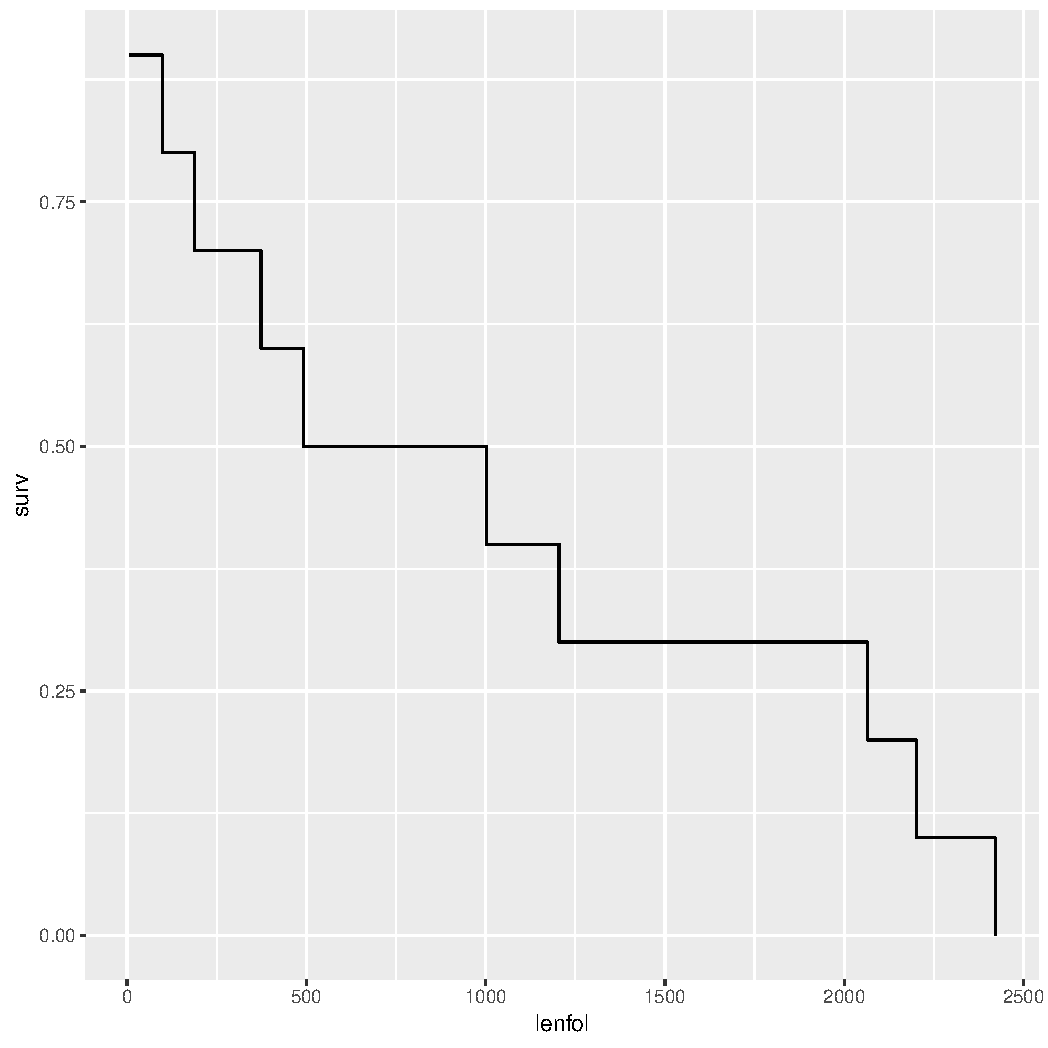
\includegraphics[scale = .3]{whas10-ecdf}
  \end{center}
  \begin{itemize}
  \item The $\hat S_e(t)$ is 1 at $t = 0$ and 0 at the final death time. %, $\max(t)$.
  \item The $\hat S_e(t)$ is assumed to be constant between adjacent death times.
  \end{itemize}
\end{frame}

\begin{frame}[fragile]
  \frametitle{Empirical survival function}
  \begin{itemize}
  \item Putting everything together, we could plot the empirical survival curve for all the uncensored subjects in \code{whas100}:
  \end{itemize}
\begin{knitrout}\scriptsize
\definecolor{shadecolor}{rgb}{0.969, 0.969, 0.969}\color{fgcolor}\begin{kframe}
\begin{alltt}
\hlstd{> }\hlstd{whas100} \hlopt \hlkwd{filter}\hlstd{(fstat} \hlopt{>} \hlnum{0}\hlstd{)} \hlopt \hlkwd{mutate}\hlstd{(}\hlkwc{surv} \hlstd{=} \hlnum{1} \hlopt{-} \hlkwd{ecdf}\hlstd{(lenfol)(lenfol))} \hlopt
\hlstd{+ }    \hlkwd{ggplot}\hlstd{(}\hlkwd{aes}\hlstd{(lenfol, surv))} \hlopt{+} \hlkwd{geom_step}\hlstd{()} \hlopt{+} \hlkwd{geom_smooth}\hlstd{()}
\end{alltt}
\end{kframe}
\end{knitrout}
  \begin{center}
    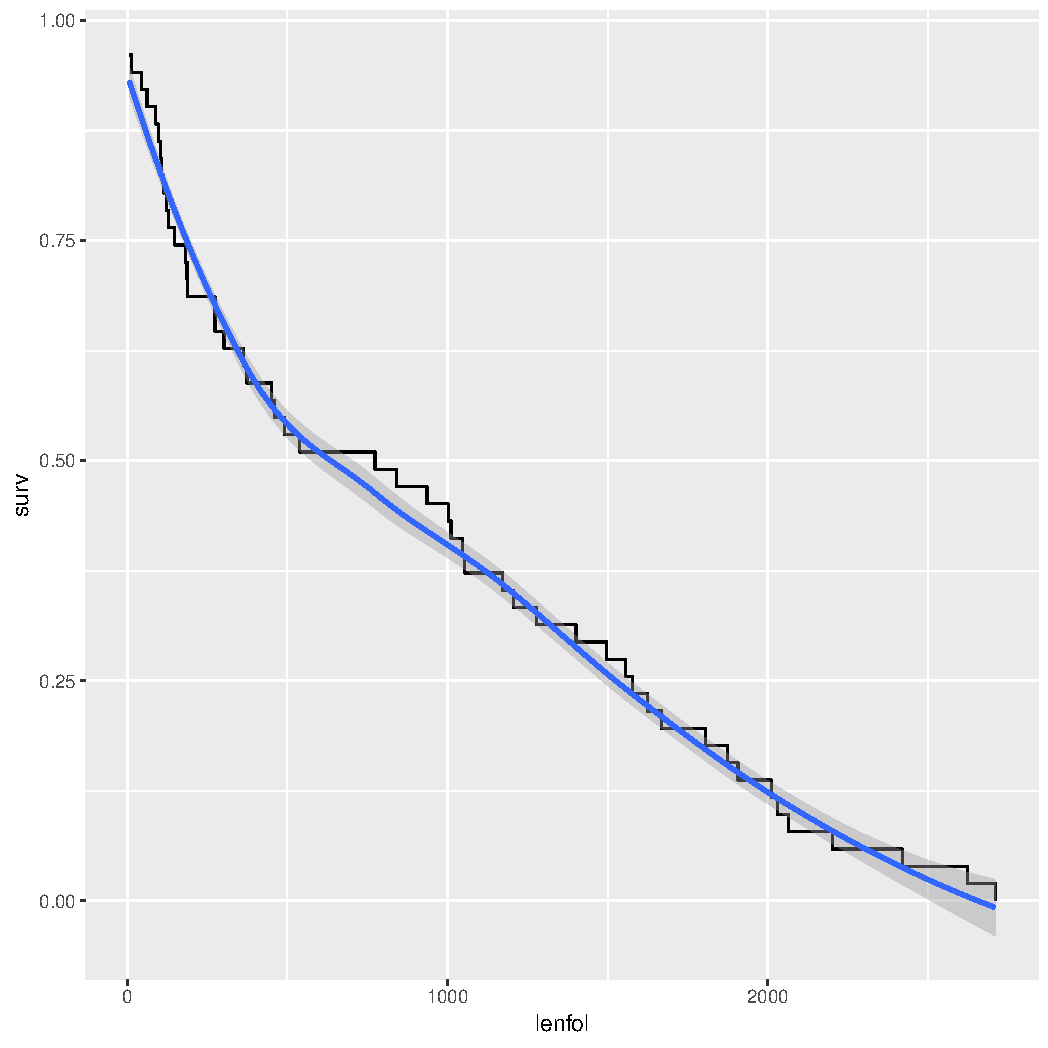
\includegraphics[scale = .3]{whas100-ecdf}
  \end{center} \vspace{-.3cm}
  \begin{itemize}
  \item The pipeline between \code{ggplot} is ``$+$'' instead of ``\code{\%>\%}''.
  \end{itemize}
\end{frame}


\begin{frame}[fragile]
  \frametitle{Kaplan-Meier estiamtor}
  \begin{itemize}
  \item With censoring, the same idea can be applied with proper adjustment.
  \item Kaplan-Meier estimator is the default estimator used by many packages. 
  \item The basic idea is to decompose $\p(T > t)$ by conditioning on prior times.
  \item Suppose a sample size of $n$, $\p(T>t)$ can be decomposed as
    {\scriptsize
    \begin{equation*}
      \Skm(t) \doteq   \p(T > t) = 
      \p(T > t_{(0)}) \cdot \p(T > t_{(1)} | T > t_{(0)}) \cdot \p(T > t_{(2)} | T > t_{(1)}) 
      \cdot\ldots\cdot \p(T > t | T > t_{(i)}),
    \end{equation*}}
    for a series of time intervals $0 \doteq  t_{(0)} < t_{(1)} < \ldots < t_{(i)} < t$ for some $i\le n$.
  \item In general, the series $\{t_{(1)}, \ldots, t_{(m)}\}$ 
    denotes the $m$ ordered death times.
  \end{itemize}
\end{frame}

\begin{frame}
  \frametitle{Kaplan-Meier estiamtor}
  Suppose we want $\p(T > 800)$ among the first 20 patients in \texttt{whas1000}.
  \begin{columns}
    \column{0.45\textwidth}
    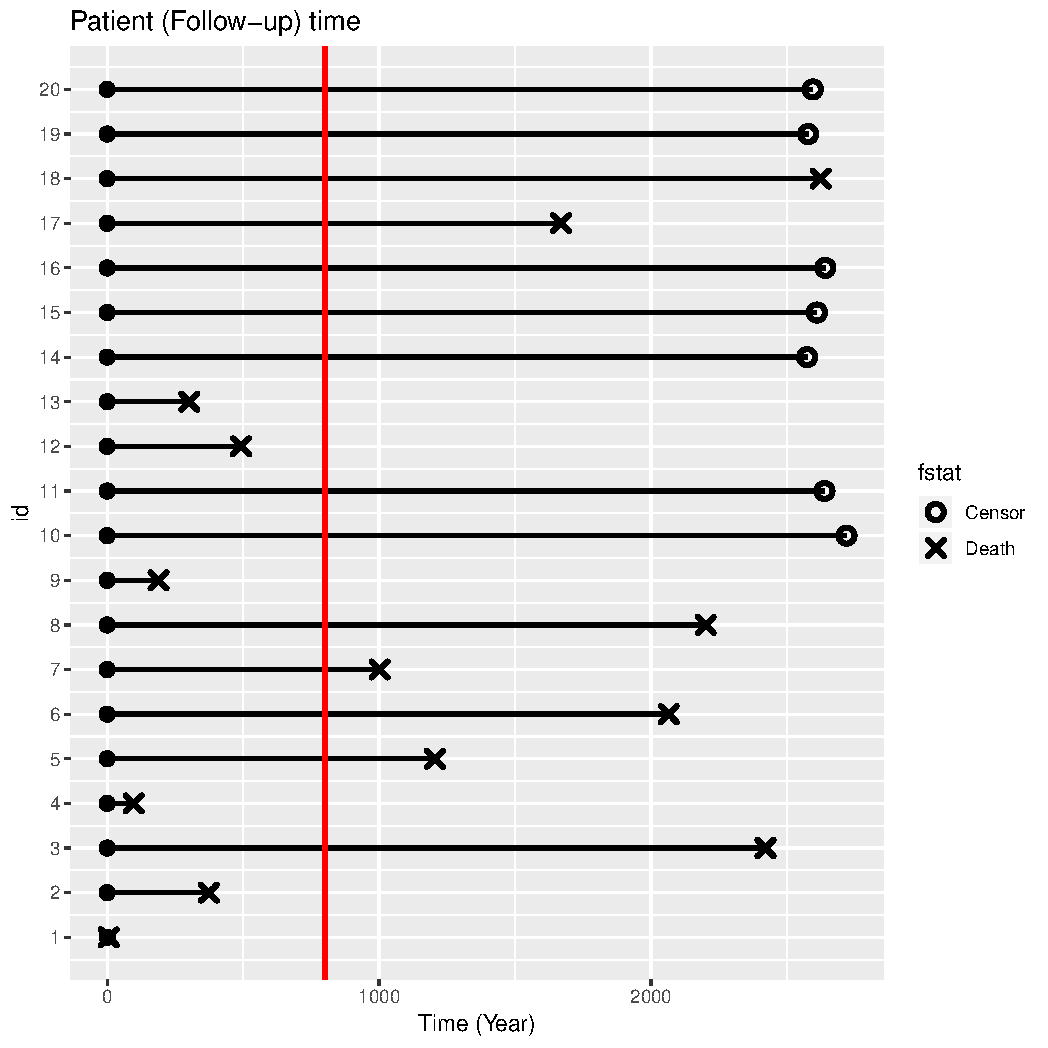
\includegraphics[scale = .3]{tab1-1-4}
    \column{0.55\textwidth}
    \begin{itemize}
    \item There are 6 events before $t = 800$.
    \item The events occured at 
      {\scriptsize
      \begin{tabular}{lllllll}
        $t_{(0)}$ & $t_{(1)}$ & $t_{(2)}$ & $t_{(3)}$ & $t_{(4)}$ & $t_{(5)}$ & $t_{(6)}$ \\
        \midrule
        0 & 6 & 98 & 189 & 302 & 374 & 492 \\
      \end{tabular}}
    \end{itemize}
  \end{columns}
  \vspace{-.3cm}
  {\scriptsize
  \begin{align*}
    \Skm(800) &= \p(T > 800) =\\
    &= \p(T > 0) \times \p(T > 6|T > 0) \times \p(T > 98|T > 6) \times
    \ldots\times \p(T > 492|T > 374) \\
    &=1 \times \frac{19}{20} \times \frac{18}{19} \times \frac{17}{18} \times \frac{16}{17} \times \frac{15}{16} \times 
    \frac{14}{15} = \frac{14}{20} = 70\%
  \end{align*}
  }
  $\Skm(800) = \hat S_e(800)$ here, why?
\end{frame}

\begin{frame}[fragile]
  \frametitle{Kaplan-Meier estimator}
  \begin{itemize}
  \item The Kaplan-Meier estimator can be obtained with the \code{survfit} function.
    % from \pkg{survival}.
\begin{knitrout}\scriptsize
\definecolor{shadecolor}{rgb}{0.969, 0.969, 0.969}\color{fgcolor}\begin{kframe}
\begin{alltt}
\hlstd{> }\hlkwd{library}\hlstd{(survival)}
\hlstd{> }\hlstd{km} \hlkwb{<-} \hlkwd{survfit}\hlstd{(}\hlkwd{Surv}\hlstd{(lenfol, fstat)} \hlopt{~} \hlnum{1}\hlstd{,} \hlkwc{data} \hlstd{= whas100,} \hlkwc{subset} \hlstd{= id} \hlopt{<=} \hlnum{20}\hlstd{)}
\hlstd{> }\hlkwd{summary}\hlstd{(km)}
\end{alltt}
\begin{verbatim}
Call: survfit(formula = Surv(lenfol, fstat) ~ 1, data = whas100, subset = id <= 
    20)

 time n.risk n.event survival std.err lower 95% CI upper 95% CI
    6     20       1     0.95  0.0487        0.859        1.000
   98     19       1     0.90  0.0671        0.778        1.000
  189     18       1     0.85  0.0798        0.707        1.000
  302     17       1     0.80  0.0894        0.643        0.996
  374     16       1     0.75  0.0968        0.582        0.966
  492     15       1     0.70  0.1025        0.525        0.933
 1002     14       1     0.65  0.1067        0.471        0.897
 1205     13       1     0.60  0.1095        0.420        0.858
 1669     12       1     0.55  0.1112        0.370        0.818
 2065     11       1     0.50  0.1118        0.323        0.775
 2201     10       1     0.45  0.1112        0.277        0.731
 2421      9       1     0.40  0.1095        0.234        0.684
 2624      4       1     0.30  0.1194        0.138        0.654
\end{verbatim}
\end{kframe}
\end{knitrout}
  \end{itemize}    
\end{frame}

\begin{frame}[fragile]
  \frametitle{Kaplan-Meier estimator}
  \begin{itemize}
  \item The Kaplan-Meier curve can be plotted with \code{plot} or \code{ggsurvplot}.
\begin{knitrout}\scriptsize
\definecolor{shadecolor}{rgb}{0.969, 0.969, 0.969}\color{fgcolor}\begin{kframe}
\begin{alltt}
\hlstd{> }\hlkwd{library}\hlstd{(survminer)}
\hlstd{> }\hlkwd{plot}\hlstd{(km)}
\hlstd{> }\hlkwd{ggsurvplot}\hlstd{(km)}
\end{alltt}
\end{kframe}
\end{knitrout}
    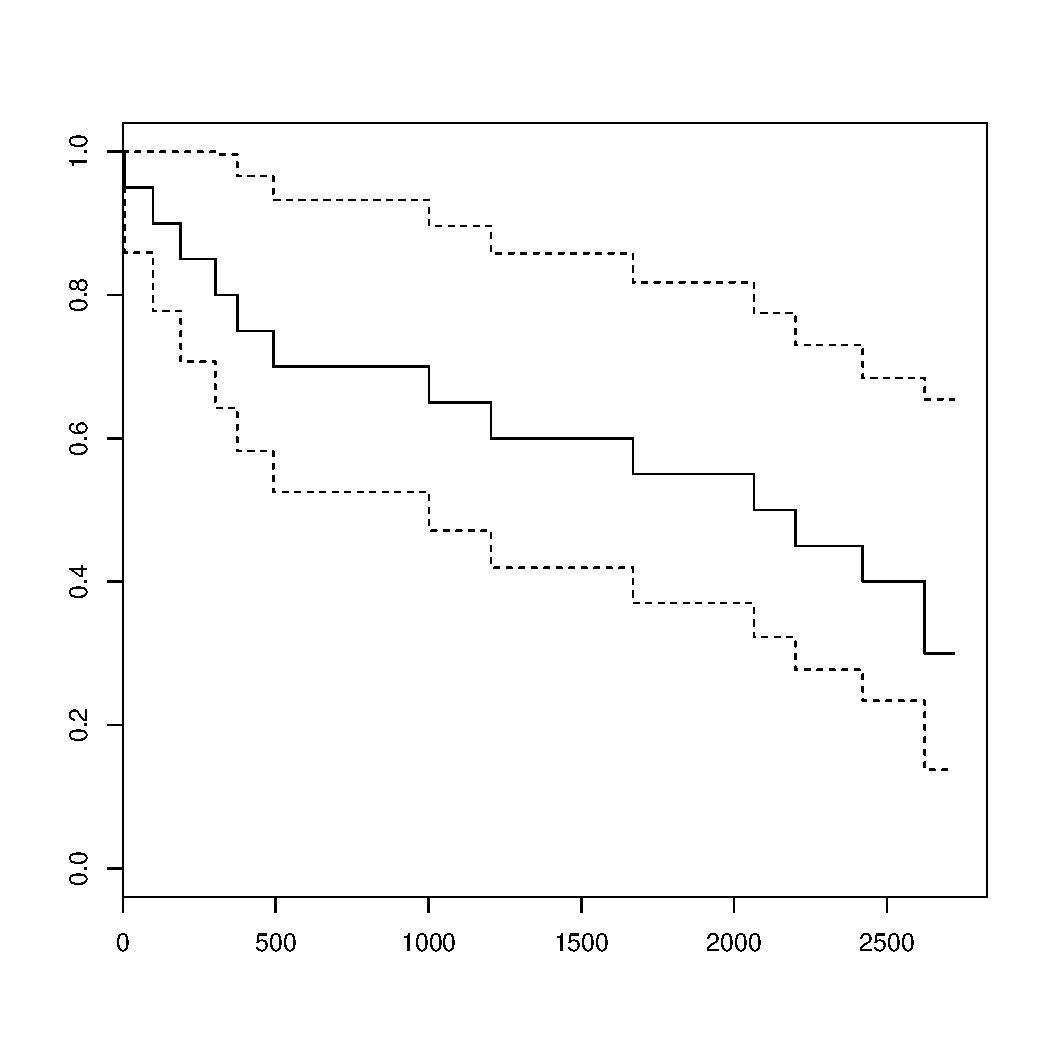
\includegraphics[scale = .28]{km1}\hspace{.2cm}
    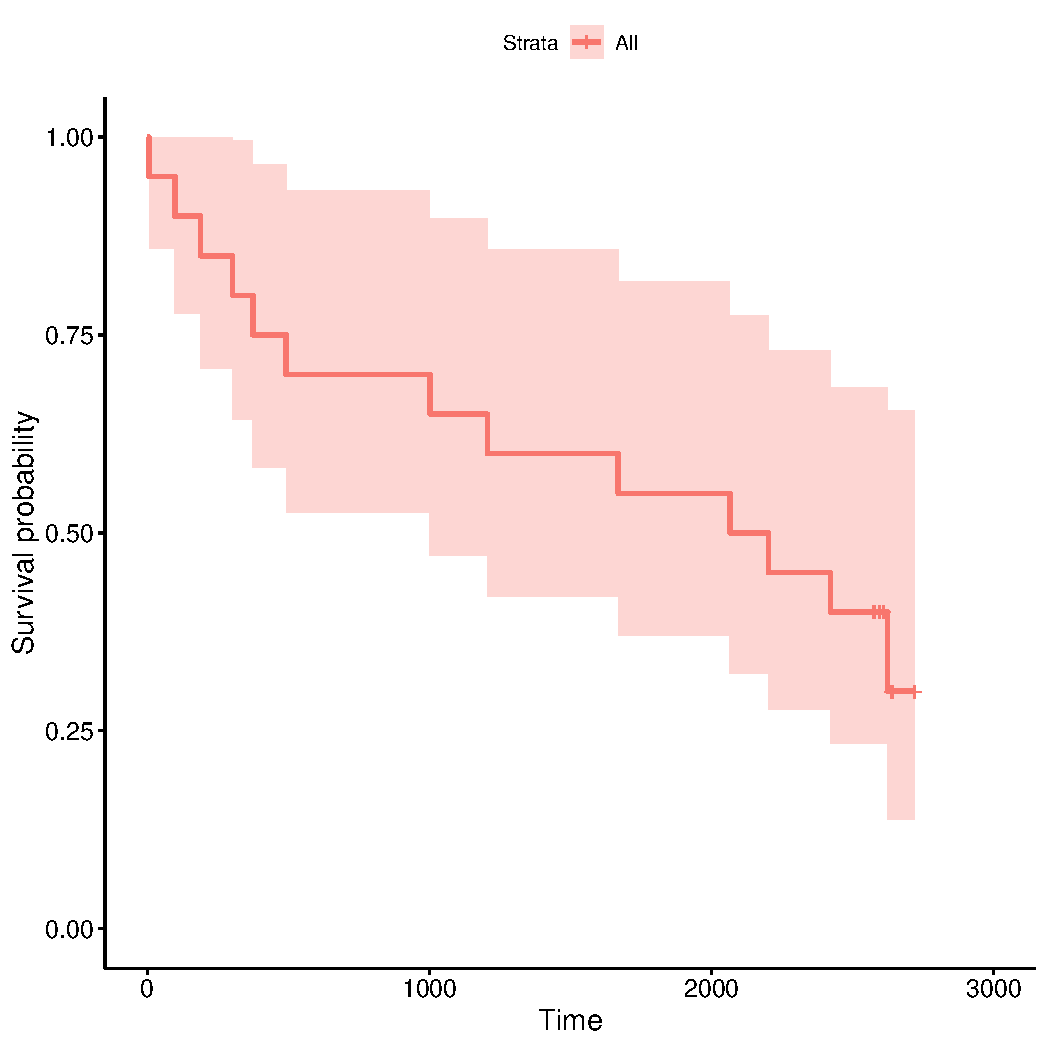
\includegraphics[scale = .28]{km2}
  \item Since \pkg{survminer} depends on the newest version of \pkg{survMisc},
    you might need to update the latter to be able to use \code{ggsurvplot}.
  \end{itemize}
\end{frame}

\begin{frame}
  \frametitle{Kaplan-Meier estimator}
  Suppose we want $\p(T > 800)$ based on the following modified data:
  \begin{columns}
    \column{0.45\textwidth}
    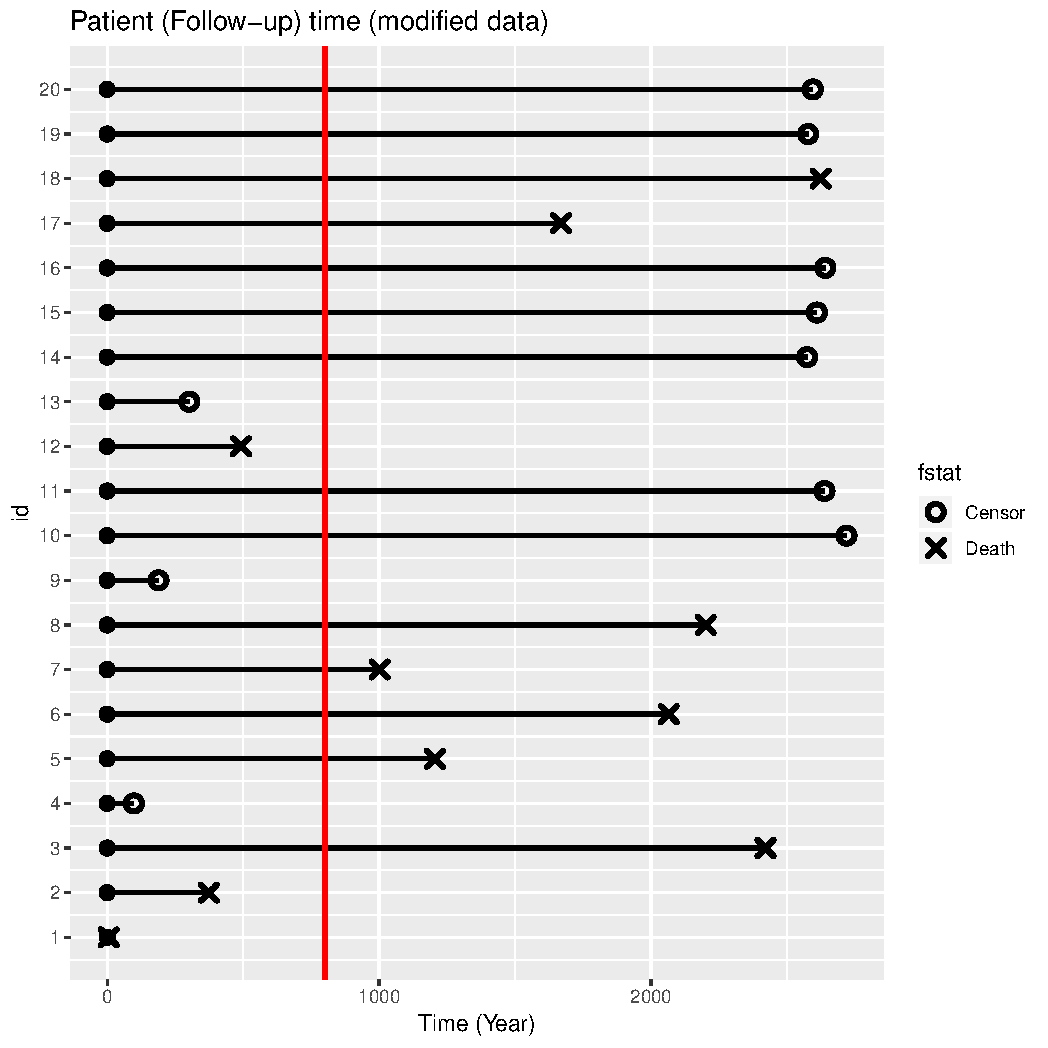
\includegraphics[scale = .3]{tab1-1-5}
    \column{0.55\textwidth}
    \begin{itemize}
    \item There are 3 events before $t = 800$.
    \item The events occured at 
      {\scriptsize
      \begin{tabular}{lllllll}
        $t_{(0)}$ & $t_{(1)}$ & $t_{(2)}$ & $t_{(3)}$ \\
        \midrule
        0 & 6 & 374 & 492 \\
      \end{tabular}}
    \item In this modified data, $t = 98, 189, 302$ are considered as censored.
    \end{itemize}
  \end{columns}
  \vspace{-.3cm}
  {\scriptsize
  \begin{align*}
    \Skm(800) &= \p(T > 800) =\\
    &= \p(T > 0) \times \p(T > 6|T > 0) \times \p(T > 374|T > 6) \times \p(T > 492|T > 374) \\
    &=1 \times \frac{19}{20} \times \frac{15}{16} \times \frac{14}{15} \approx 83.1\%
  \end{align*}
  }
\end{frame}

\begin{frame}[fragile]
  \frametitle{Kaplan-Meier estimator}
  \begin{itemize}
  \item The Kaplan-Meier estimator for the whole data is
\begin{knitrout}\scriptsize
\definecolor{shadecolor}{rgb}{0.969, 0.969, 0.969}\color{fgcolor}\begin{kframe}
\begin{alltt}
\hlstd{> }\hlkwd{library}\hlstd{(survival)}
\hlstd{> }\hlstd{km} \hlkwb{<-} \hlkwd{survfit}\hlstd{(}\hlkwd{Surv}\hlstd{(lenfol, fstat)} \hlopt{~} \hlnum{1}\hlstd{,} \hlkwc{data} \hlstd{= whas100)}
\hlstd{> }\hlkwd{plot}\hlstd{(km)}
\hlstd{> }\hlkwd{ggsurvplot}\hlstd{(km)}
\end{alltt}
\end{kframe}
\end{knitrout}
    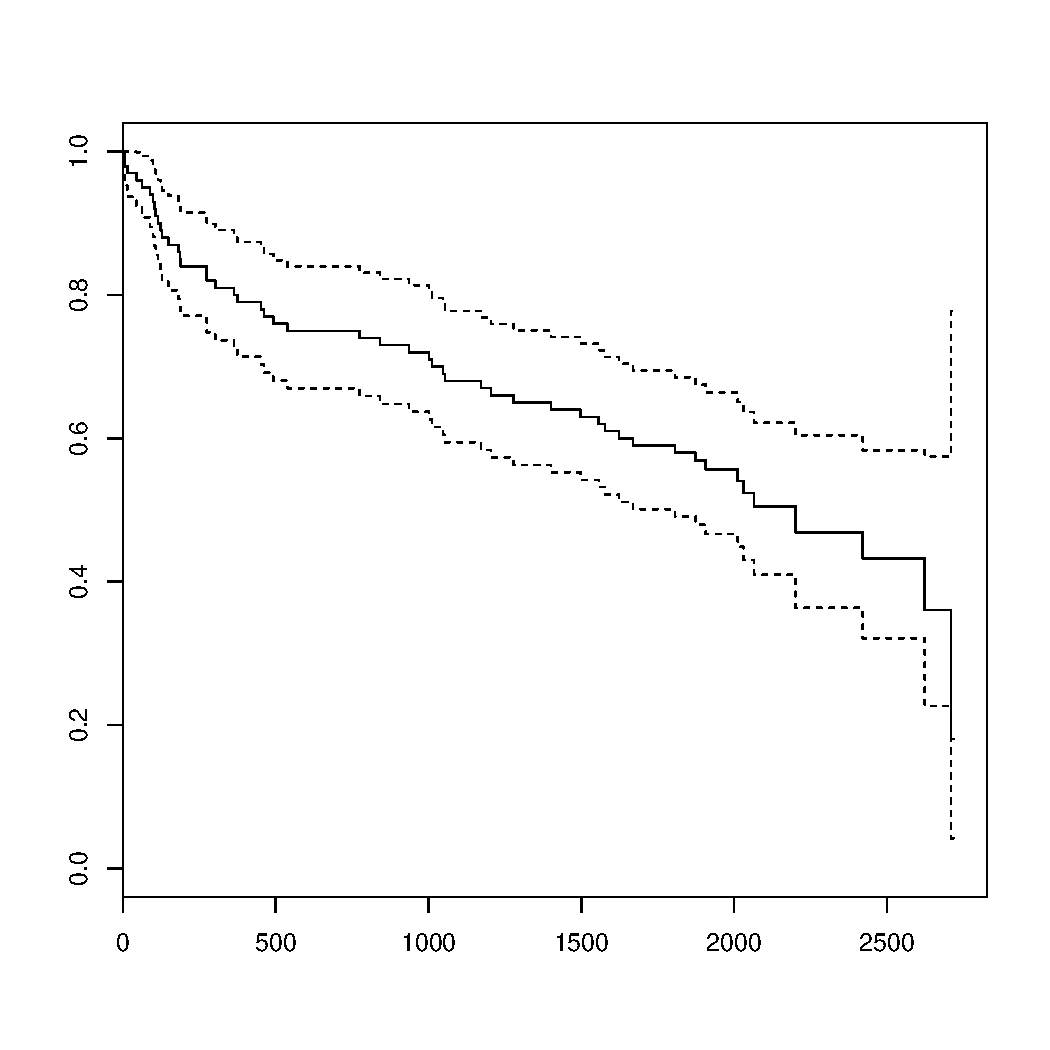
\includegraphics[scale = .28]{km3}\hspace{.2cm}
    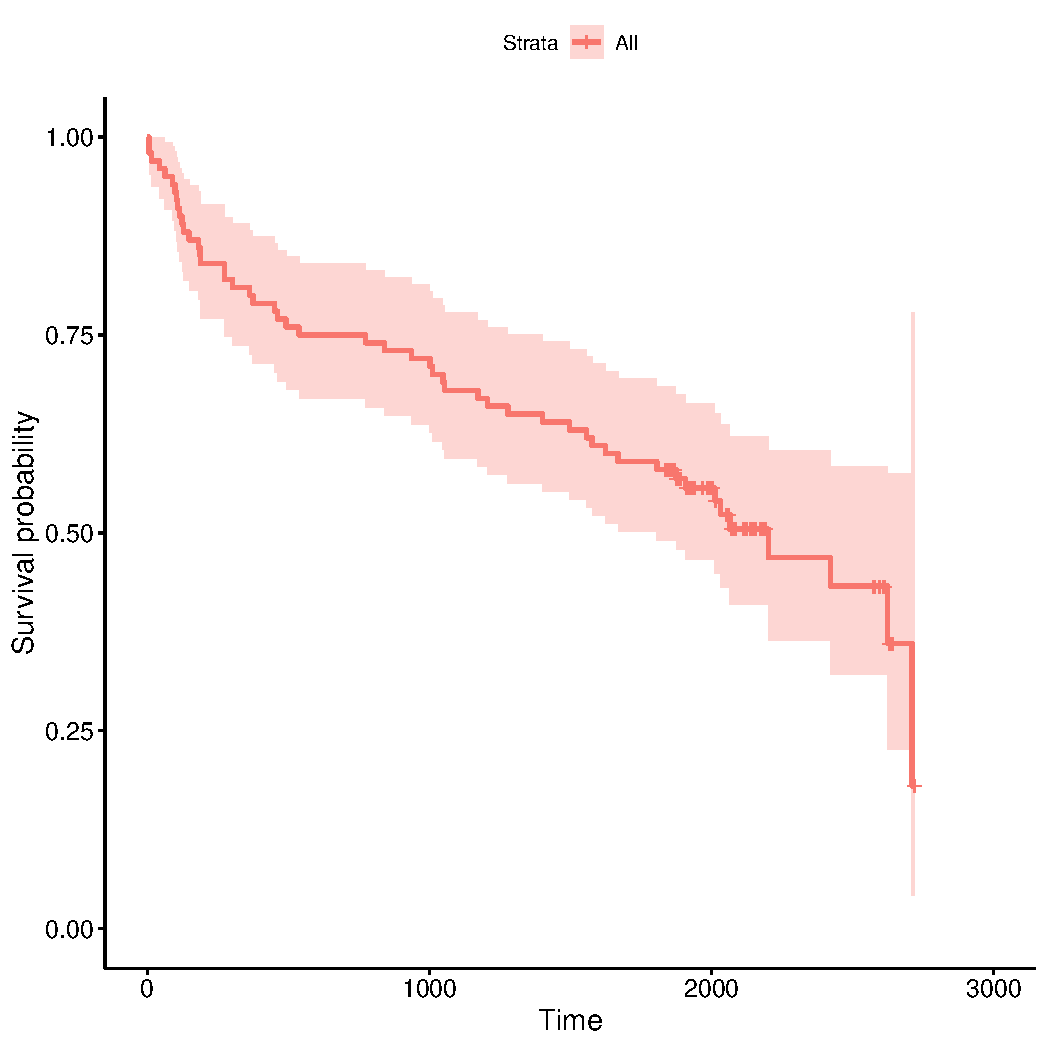
\includegraphics[scale = .28]{km4}
  \item If the last observed time corresponds to a censored observation, 
    then the estimate of the survival function does not go to zero.
  \end{itemize}    
\end{frame}


\begin{frame}
  \frametitle{Kaplan-Meier estimator}
  \begin{itemize}
  \item Suppose we have a sample of $n$ independent observations $(t_i, c_i), i = 1, 2, \ldots, n$.
  \item Suppose there are $m$ deaths and $m\le n$.
  \item The series $\{t_{(1)}, \ldots, t_{(m)}\}$ are the $m$ ordered death times.
  \item The Kaplan-Meier estimator has the form
    \begin{equation*}
      \Skm(t) = \prod_{t_{(i)} \le t}\frac{n_i - d_i}{n_i} = \prod_{t_{(i)} \le t} 1 - \frac{d_i}{n_i},
    \end{equation*}
    where $n_i$ is the number of individual who are alive at $t_{(i)}$ (at risk),
    and $d_i$ is the number of individual who died at $t_{(i)}$.
  \item A potential problem with the Kaplan-Meier estimator is when $n_i$ is small and
    $n_i = d_i$ occurs at early time.
  \end{itemize}    
\end{frame}

\begin{frame}
  \frametitle{Nelson-Aalon estimator}
  \begin{itemize}
  \item An alternative estimate of $\Skm(t)$ is the \empr{Nelson-Aalon estimator}:
    \begin{equation*}
      \Sna(t) = \prod_{t_{(i)} \le t} \exp\left(-\frac{d_i}{n_i}\right).
    \end{equation*}
  \item The main idea is to see $d_i/n_i$ as the event rate, i.e., $h(t_{(i)}) = d_i/n_i$.
  \item Recall the relationship $h(t) = f(t) / S(t)$ and think of $d_i/n$ and $n_i/n$ 
    are raw estimates of $f(t)$ and $S(t)$.
  \item By the similar argument, we have
    $$\Hna(t) \doteq H(t) = \sum_{t_{(i)} \le t} d_i/n_i, \mbox{ and } S(t) = e^{-\Hna(t)} = \Sna(t).$$
  \item $\Sna(t)$ and $\Skm(t)$ are derived differently, but both based on $d_i$ and $n_i$.
  \item In general $\Sna(t)\ge\Skm(t)$ but $\Sna(t)\approx\Skm(t)$.
  \end{itemize}
\end{frame}

\begin{frame}[fragile]
  \frametitle{Nelson-Aalon estimator}
  \begin{itemize}
  \item $\Sna(t)$ has slightly nicer properties and is more stable.
  \item If the interest is in estimating the cumulative hazard function, $H(t)$, 
    we can use either the $\Hna(t)$, or $\Hkm(t) = -\log\Skm(t)$.
  \item The $\Hkm(t)$ follows directly form from $\Skm(t)$:
    \begin{equation*}
      \Hkm(t) = - \sum_{t_{(i)}\le t}\log\left(\frac{n_i - d_i}{n_i}\right).
    \end{equation*}
  \item Problems with this estimator? 
  \end{itemize}
\end{frame}    
    
\begin{frame}[fragile]
  \frametitle{Nelson-Aalon estimator}
  \begin{itemize}
  \item $\Sna(t)$ can be obtained with \code{coxph} of the \pkg{survival} package.
\begin{knitrout}\scriptsize
\definecolor{shadecolor}{rgb}{0.969, 0.969, 0.969}\color{fgcolor}\begin{kframe}
\begin{alltt}
\hlstd{> }\hlkwd{args}\hlstd{(coxph)}
\end{alltt}
\begin{verbatim}
function (formula, data, weights, subset, na.action, init, control, 
    ties = c("efron", "breslow", "exact"), singular.ok = TRUE, 
    robust = FALSE, model = FALSE, x = FALSE, y = TRUE, tt, method = ties, 
    ...) 
NULL
\end{verbatim}
\end{kframe}
\end{knitrout}
  \item \code{coxph} refers to ``Cox proportional hazard model'' that has the form
    \begin{equation}
      h(t) = h_0(t) e^{X^\top\beta}, 
      \label{eq:cox}
    \end{equation}
    where $X$ is the covariate matrix, $\beta$ is the regression coefficient, 
    and $h_0(t)$ is called the \empr{baseline hazard} function.
  \item More details will be given in Chapter 3. 
  \end{itemize}
\end{frame}


\begin{frame}[fragile]
  \frametitle{Nelson-Aalon estimator}
  \begin{itemize}
  \item For now, we will assume $\beta = 0$ in~\eqref{eq:cox}, which implies $h(t) = h_0(t)$.
  \item We will use $h_0(t)$ to obtain $\Sna(t)$.
\begin{knitrout}\scriptsize
\definecolor{shadecolor}{rgb}{0.969, 0.969, 0.969}\color{fgcolor}\begin{kframe}
\begin{alltt}
\hlstd{> }\hlstd{cox} \hlkwb{<-} \hlkwd{coxph}\hlstd{(}\hlkwd{Surv}\hlstd{(lenfol, fstat)} \hlopt{~} \hlnum{1}\hlstd{,} \hlkwc{data} \hlstd{= whas100)}
\hlstd{> }\hlstd{H0} \hlkwb{<-} \hlkwd{basehaz}\hlstd{(cox)}
\hlstd{> }\hlkwd{str}\hlstd{(H0)}
\end{alltt}
\begin{verbatim}
'data.frame':	95 obs. of  2 variables:
 $ hazard: num  0.0201 0.0303 0.0406 0.051 0.0616 ...
 $ time  : num  6 14 44 62 89 98 104 107 114 123 ...
\end{verbatim}
\end{kframe}
\end{knitrout}
\begin{knitrout}\scriptsize
\definecolor{shadecolor}{rgb}{0.969, 0.969, 0.969}\color{fgcolor}\begin{kframe}
\begin{alltt}
\hlstd{> }\hlkwd{plot}\hlstd{(km)}
\hlstd{> }\hlkwd{lines}\hlstd{(H0}\hlopt{$}\hlstd{time,} \hlkwd{exp}\hlstd{(}\hlopt{-}\hlstd{H0}\hlopt{$}\hlstd{hazard),} \hlstr{'s'}\hlstd{,} \hlkwc{col} \hlstd{=} \hlnum{2}\hlstd{)}
\end{alltt}
\end{kframe}
\end{knitrout}
    \begin{center}
      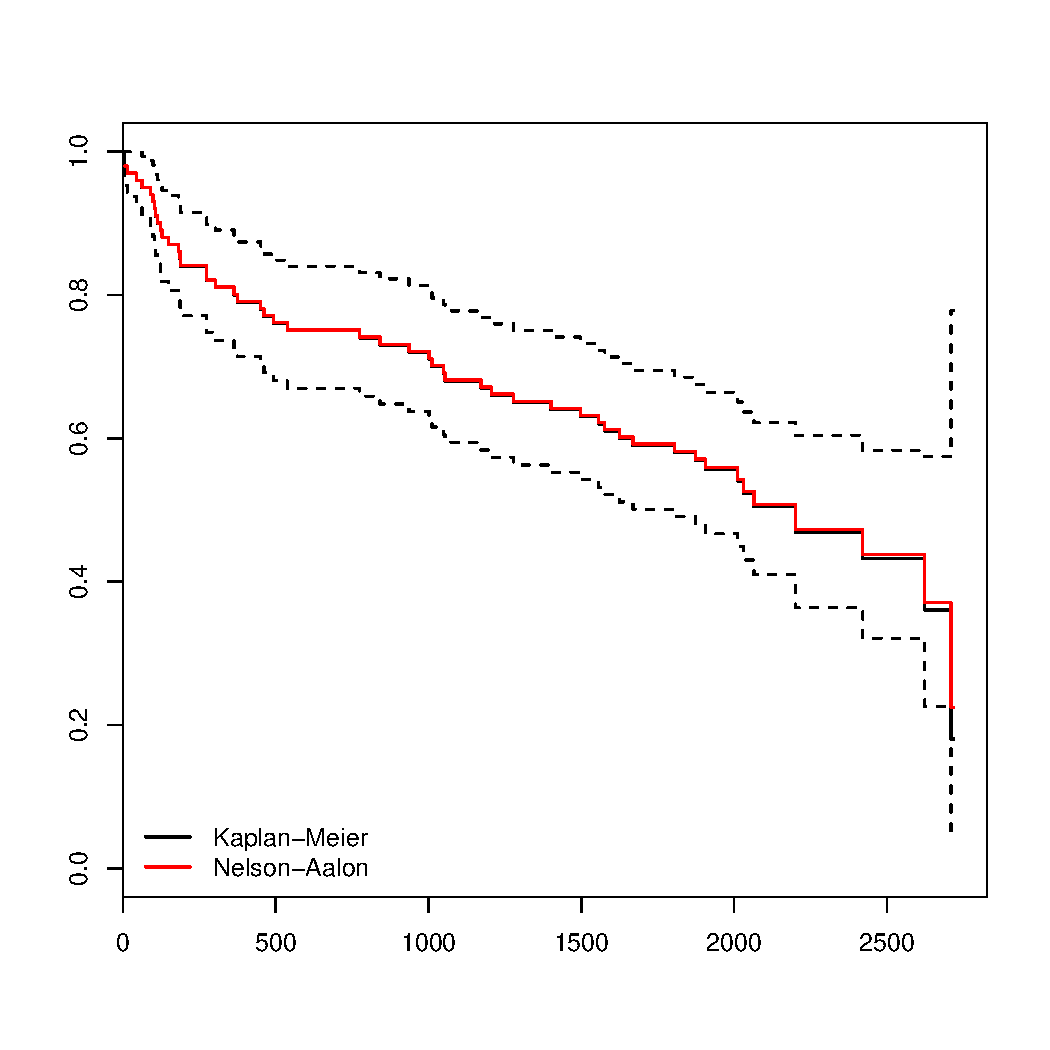
\includegraphics[scale = .25, trim = 1cm 1.6cm 1cm 2cm, clip]{km5}
    \end{center}
  \end{itemize}
\end{frame}


\begin{frame}
  \frametitle{Life-table estimates}
  \begin{itemize}
  \item When dataset is large, the $\Skm(t)$ and $\Sna(t)$ can be obtained with intervals of time, 
    rather than exact time points.
    \begin{itemize}
    \item The series $\{t_{(1)}, \ldots, t_{(m)}\}$ represents intervals. 
    \item $d_i$ represents the number of individual who died in $t_{(i)}$.
    \item $n_i$ represents the number of individual who are alive in $t_{(i)}$.
    \end{itemize}
  \item Potential problem with censoring? 
  \item Adjustments under uniform assumption (p25).
  \item Better to adopt methods for data with interval censoring.
\end{itemize}
\end{frame}

\begin{frame}
  \frametitle{Inference on $\Skm(t)$}
  \begin{itemize}
    \item The 95\% confidence interval (CI) does not follow the usual form of 
      $$\mbox{PE} \pm 1.96 \times\mbox{SE}.$$
    \item This is mainly because $\Skm(t)$ needs to lie between 0 and 1. 
    \item Two common methods to obtain the 95\% CI for $\Skm(t)$ are the
      $\log$ and $\log$-$\log$ transformations.
    \item The idea is to derive the standard errors on the transformed scale first, 
      then back-transform these back.
  \end{itemize}
\end{frame}

\section{The Delta method}
\begin{frame}
  \frametitle{The Delta Method}
  \begin{itemize}
    \item We need the Delta method to estimate the standard errors.
    \item The Delta method states that
      $$ \Var\{g(X)\}\approx \Var(X) \cdot\{g^\prime(x_0)\}^2,$$
      where $g^\prime(x_0)$ is the 1st derivative of $g(\cdot)$ evaluates at constant $x_0$.
  \end{itemize}
\end{frame}

\begin{frame}
  \frametitle{The Delta Method}
  \begin{itemize}
    \item A special case of the Delta method is when $g(\cdot) = \log(\cdot)$.
    \item Setting $g(\cdot) = \log(\cdot)$, we have
      $$ \Var\{f(X)\}\approx \frac{\Var(X)}{x_0^2}.$$
  \end{itemize}
\end{frame}

\section{Inference on $\Skm(t)$}
\begin{frame}
  \frametitle{Inference on $\Skm(t)$}
  \begin{itemize}
    \item We will first look at the $\log$ transformation.
    \item Recall $$\Skm(t) = \prod_{t_{(i)}\le t}\frac{n_i - d_i}{n_i}.$$
    \item The variance of $\log$-transformed $\Skm(t)$ gives
       $$\Var\left\{\log\Skm(t)\right\} = \Var\left\{\sum_{t_{(i)}\le t}\log\left(\frac{n_i - d_i}{n_i}\right)\right\} = 
       \sum_{t_{(i)}\le t}\Var\left\{\log\left(\frac{n_i - d_i}{n_i}\right)\right\}.$$
     \item We assume independence between observations in the risk sets.
     \item For convenience, let's write $p_i = (n_i - d_i) / n_i$, and $\hat p_i$ when $n_i$ and $d_i$ are known.
  \end{itemize}
\end{frame}


\begin{frame}
  \frametitle{Inference on $\Skm(t)$}
  \begin{itemize}
  \item The key is to estimate $\Var\left\{\log\left(p_i\right)\right\}$ with the Delta method.
  \item For each $t_{(i)}$, $n_i$ is fixed but $d_i$ is random. 
  \item $n_i - d_i$ can be assumed to follow the binomial distribution with parameters $n_i$ and $1 - d_i / n_i$.
    Then
    \begin{align*}
      % \E(p_i) &= \frac{\E(n_i - d_i)}{n_i} = 1 - \frac{d_i}{n_i}, \\
      \Var(p_i) &= \frac{\Var(n_i - d_i)}{n_i^2} = \frac{\frac{d_i}{n_i}\cdot\left(1 - \frac{d_i}{n_i}\right)}{n_i}.
    \end{align*}
  \item With the Delta method, we have
    % $$ \Var\{\log(p_i)\} \approx \frac{\Var(p_i)}{\E^2(p_i)} = \frac{d_i}{n_i\cdot(n_i-d_i)}. $$
    $$ \Var\{\log(p_i)\} \approx \frac{\Var(p_i)}{\hat p_i} = \frac{d_i}{n_i\cdot(n_i-d_i)}. $$
  \end{itemize}
\end{frame}


\begin{frame}
  \frametitle{Inference on $\Skm(t)$}
  \begin{itemize}
  \item From the above result, we have
    $$\Var\left\{\log\Skm(t)\right\} \approx \sum_{t_{(i)}\le t}\frac{d_i}{n_i\cdot(n_i-d_i)}. $$
  \item By the Delta method (again), 
    $$\Var\left\{\log\Skm(t)\right\} \approx \Var\{\Skm(t)\} \cdot \frac{1}{\Skm^2(t)}.$$ 
  \item Altogether, this gives
    $$ \Var\{\Skm(t)\} \approx \Skm^2(t)\cdot\sum_{t_{(i)}\le t}\frac{d_i}{n_i\cdot(n_i-d_i)}.$$
  \item This result is known as the \empr{Greenwood's formula}, or the $\log$ transformation.
  \item This estimator can be obtained from a counting process approach.
  \end{itemize}
\end{frame}


\begin{frame}
  \frametitle{Inference on $\Skm(t)$}
  \begin{itemize}
  \item The Greenwood formula is the default method for \texttt{survfit}.
  \item With the Greenwood formula, the $100(1- \alpha)\%$ condifdence interval of $\Skm(t)$ can be obtained using the usual form of $\mbox{PE}\pm Z_{\alpha/2}\times\mbox{SE}$.
  \item The bounds can still be outside of $[0, 1]$.
  \item An alternative approach is to consider the $\log$-$\log$ transformation.
  \end{itemize}
\end{frame}


\begin{frame}
  \frametitle{Inference on $\Skm(t)$}
  \begin{itemize}
  \item By the Delta method, we have
    % $\log$-$\log$ transformation considers
    \begin{equation*}
      \Var\left[\log\left\{-\log \Skm(t)\right\}\right] \approx 
      % \frac{\Var\left[\log\Skm(t)\right]}{\left\{-\log\Skm(t)\right\}^2}
      \frac{1}{\{-\log\Skm(t)\}^2} \cdot\sum_{t_{(i)}\le t}\frac{d_i}{n_i\cdot(n_i-d_i)}.
    \end{equation*}
  \item This imples that the $100(1- \alpha)\%$ condifdence interval can be constructed by inversing 
    \begin{equation*}
      \log\{-\log\Skm(t)\} \pm Z_{\alpha/2} \times \SE\left[\log\{-\log\Skm(t)\}\right]
    \end{equation*}
  \item Since $-\log$ of a survival function gives the cumulative hazard function, e.g., $-\log S(t) = H(t)$, 
    the $\log$-$\log$ approach called the ``$\log$ hazard'' approach. 
  \end{itemize}
\end{frame}

\begin{frame}[fragile]
  \frametitle{Inference on $\Skm(t)$}
  \begin{itemize}
  \item Types of CI can be specified with \code{conf.type} in \code{survfit}.
\begin{knitrout}\scriptsize
\definecolor{shadecolor}{rgb}{0.969, 0.969, 0.969}\color{fgcolor}\begin{kframe}
\begin{alltt}
\hlstd{> }\hlopt{?}\hlstd{survfit.coxph}
\end{alltt}
\end{kframe}
\end{knitrout}
  \item Some options are available for \code{conf.type} depending on $g(\cdot)$ used in the Delta method.
    \begin{description}
    \item[\code{plain}] $g(x) = x$
      \item[\code{log}] $g(x) = \log(x)$
      \item[\code{log-log}] $g(x) = \log\{-\log(x)\}$
      \item[\code{logit}] $g(x) = \log\left(\frac{x}{1 - x}\right)$
      \item[\code{arcsin}] $g(x) = \arcsin\sqrt(x)$
      \end{description}
  \item In addition, \citet{peto1977design} proposed to estimate $\Var\{\Skm(t)\}$ from
    \begin{equation*}
      \Var\{\Skm(t)\} = \frac{\Skm(t) \cdot (1 - \Skm(t))}{n_i}
    \end{equation*}
  \end{itemize}
\end{frame}

\begin{frame}
\frametitle{Inference on $\Skm(t)$}
  \begin{itemize}
    \item The following depict $\Skm(t)$ with the five \code{conf.type}'s for \code{whas100}.
    \item The CI's are quite close to each other.
  \end{itemize}
  \begin{center}
    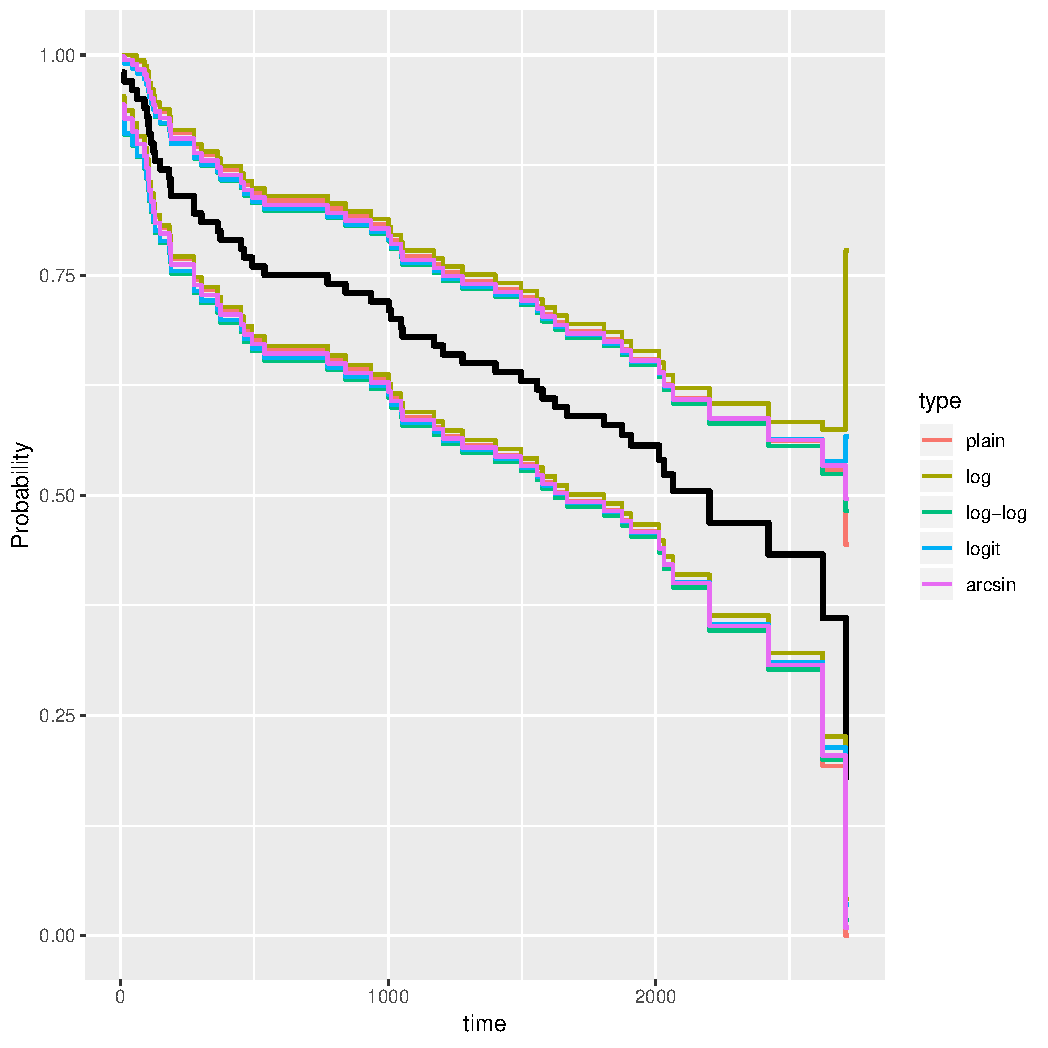
\includegraphics[height = 5.7cm]{kmplot} \hspace{.02cm}
    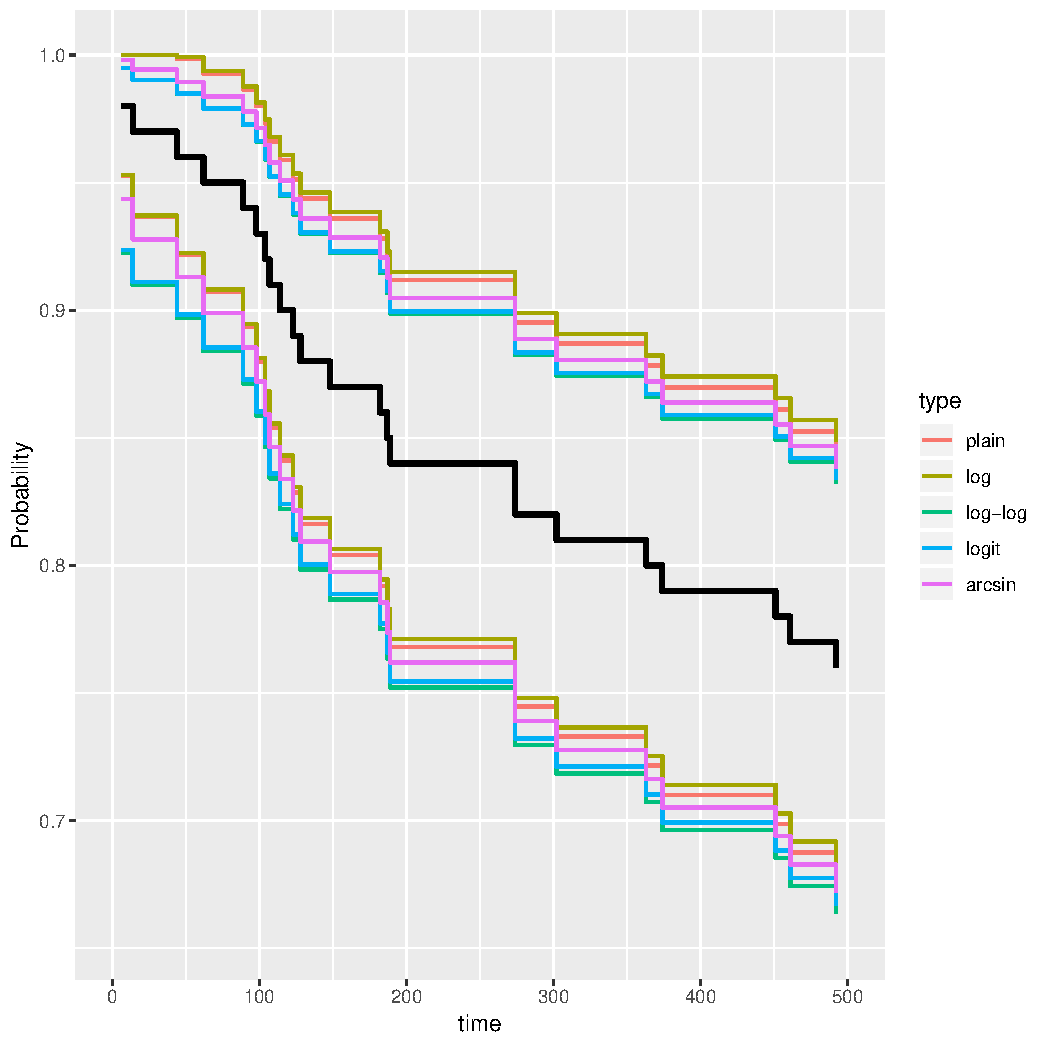
\includegraphics[height = 5.7cm]{kmplot2}
  \end{center}
\end{frame}

\section{Median and percentiles}
\begin{frame}
  \frametitle{*Inference on the median and percentiles}
  \begin{itemize}
  \item Given a $\Ss(t)$ ($\Skm(t)$ or $\Sna(t)$), the estimate of the $p$th percentile is 
    $$ \tp = \min\{t: \hat{S}(t) \le (p / 100)\}.$$
  \item The Delta method can be used again to obtain $\Var(\tp)$.
  \item Setting $g(\cdot) = S(\cdot)$, we have the relationship
    \begin{equation*}
    \Var\{\Ss(\tp)\} \approx \Var(\tp) \cdot \{f(\tp)\}^2,
    \label{eq:mp}
    \end{equation*}
    where $f(t) = \dif \Ss(t) / \dif t$.
  \item The only unknown in the above equation is $f(t)$, 
    which can be approximated by linear interpolation:
    $$\hat f(\tp) \approx\frac{\Ss(\hat u_p) - \Ss(\hat l_p)}{\hat l_p - \hat u_p}, $$
    where $\hat u_p < \tp < \hat l_p$, $\hat u_p = \max\{t:\Ss(t) \ge p / 100 + \epsilon\}$ and 
    $\hat l_p = \min\{t:\Ss(t) \le p / 100 - \epsilon\}$, for some small constant $\epsilon$.
  \end{itemize}
\end{frame}

\begin{frame}[fragile]
  \frametitle{*Inference on the median and percentiles}
  \begin{itemize}
  \item Replacing the unknown quantities with their empirical estimates, 
    the $100(1-\alpha)$\% CI can be obtained through
    $\tp \pm Z_{\alpha/2}\times\SE(\tp)$.
  \item Clinicians are specifically interested in median survival (follow-up) time, 
    because survival time data often tend to skewed to the right.
  \item Other quantity of interest is the semi-interquartiles range (SIQR):
    $$\mbox{SIQR} = \frac{t_{75} - t_{25}}{2}.$$
  \item Like the variance, the larger the SIQR, the more dispersed is the survival time distribution.
  \end{itemize}
\end{frame}

\begin{frame}[fragile]
  \frametitle{*Inference on the median and percentiles}
  \begin{itemize}  
  \item Median survival time is printed by \code{survfit}.
\begin{knitrout}\scriptsize
\definecolor{shadecolor}{rgb}{0.969, 0.969, 0.969}\color{fgcolor}\begin{kframe}
\begin{alltt}
\hlstd{> }\hlkwd{survfit}\hlstd{(}\hlkwd{Surv}\hlstd{(lenfol, fstat)} \hlopt{~} \hlnum{1}\hlstd{,} \hlkwc{data} \hlstd{= whas100)}
\end{alltt}
\begin{verbatim}
Call: survfit(formula = Surv(lenfol, fstat) ~ 1, data = whas100)

      n  events  median 0.95LCL 0.95UCL 
    100      51    2201    1806      NA 
\end{verbatim}
\end{kframe}
\end{knitrout}
  \item Median follow-up time does not always exists.
\begin{knitrout}\scriptsize
\definecolor{shadecolor}{rgb}{0.969, 0.969, 0.969}\color{fgcolor}\begin{kframe}
\begin{alltt}
\hlstd{> }\hlkwd{survfit}\hlstd{(}\hlkwd{Surv}\hlstd{(lenfol, fstat)} \hlopt{~} \hlnum{1}\hlstd{,} \hlkwc{data} \hlstd{= whas100[}\hlnum{81}\hlopt{:}\hlnum{100}\hlstd{,])}
\end{alltt}
\begin{verbatim}
Call: survfit(formula = Surv(lenfol, fstat) ~ 1, data = whas100[81:100, 
    ])

      n  events  median 0.95LCL 0.95UCL 
     20       9      NA    1577      NA 
\end{verbatim}
\end{kframe}
\end{knitrout}
  \item A more practical approach?
  \end{itemize}
\end{frame}

\section{Introduction to Counting Processes}
\begin{frame}
  \frametitle{Counting processes}
  \begin{itemize}  
  \item As is seen from before, the focus in survival analysis is on observing the occurrence of events over time. 
  \item Such occurrences constitute point (counting) process; counting number of events as they come along. 
  \item There is a very neat collection of theories for counting processes.
  \item More in-depth details can be found in \citet{fleming2011counting,kalbfleisch2011statistical}.
  \end{itemize}    
\end{frame}

\begin{frame}
  \frametitle{Counting processes}
  \begin{itemize}  
  \item Appendix 2 gives a short introduction of counting processes, in the case of right censoring. 
  \item We start by focusing on a \empr{single type} of event without censoring.
  \item For a given time $t$, let $N(t)$ be the number of events over the time period $(0, t]$, 
    then $N(t)$ is a counting process.
  \item The counting process $N(t)$ is \empr{continuous from the right}, with jump size 1.
  \end{itemize}    
\end{frame}


\begin{frame}
  \frametitle{Poisson process}
  \begin{itemize}  
  \item A well-known example of a counting process is the homogeneous Poisson process.
  \item Jumps occur randomly and independently of each other (independent increment property).
  \item A homogeneous Poisson process is described by its \empr{intensity} $\lambda$.
  \item The $\lambda$ is the probability of occurrence of an event in a small interval divided by the length of the interval.
  \item We will apply this idea to modeling counting process.
  \end{itemize}    
\end{frame}

\begin{frame}
  \frametitle{Counting processes}
  \begin{itemize}  
  \item Suppose the intensity function that describes $N(t)$ is $\lambda(t)$.
  \item Under our assumption that a subject can experience at most one event, 
    consider a small time interval $[t, t + \dt)$,
    $\lambda(t)$ is
    \begin{equation*}
      \lambda(t) \dt = \p(\dif N(t) = 1|\mbox{past}),
    \end{equation*}
    where $\dif N(t)$ denotes the \# of events in $[t, t + dt)$, or $N(t + \dt) - N(t)$.
  \item Formally speaking, the ``past'' represents the \empr{filtration} of the process up to but not including time $t$.
  \end{itemize}    
\end{frame}


\begin{frame}
  \frametitle{Counting processes}
  \begin{itemize}  
  \item Under our assumption, $\dif N(t)$ is binary, and 
    $$\lambda(t) \dt = \E\{\I(\dif N(t) = 1)|\mbox{past}\} = \E\{\dif N(t)|\mbox{past}\}.$$
  \item Then it follows
    \begin{equation}
      \label{eq:Emart}
      \E(\dif N(t) - \lambda(t) \dt |past) = 0.
    \end{equation}
  \item If we define a new process 
    \begin{equation}
      \label{eq:mart}
      M(t) = N(t) - \int_0^t\lambda(s) \dif s,
    \end{equation}
    then we have $\E(\dif M(t) | past) = 0$.
  \item It turns out $M(t)$ is a zero-mean martingale.
  \end{itemize}
\end{frame}

\begin{frame}
  \frametitle{Counting processes}
  \begin{itemize}  
  \item Definition~\eqref{eq:mart} can be written as
    \begin{equation}
      \dif N(t) = \lambda(t) \dif t + \dif M(t),
      \label{eq:mart2}
    \end{equation}
    reflecting the relationship \empr{observation = signal + noise}.
  \item Think of $M(t)$ as the sum of random errors.
  \item Let 
    $$\Lambda(t) = \int_0^t\lambda(s)\dif s,$$
    \eqref{eq:Emart} and~\eqref{eq:mart} implies $\Lambda(t)$ is the cumulative expected \# of events in $(0, t]$, 
    or $\Lambda(t) = \E\{N(t)\}$.
  \item $\Lambda(t)$ versus $H(t)$?
  \end{itemize}
\end{frame} 

\begin{frame}
  \frametitle{Counting processes}
  \begin{itemize}  
  \item Now we will look at the scenario when there is only \empr{one event type} and a subject can experience \empr{at most one event} (no ties in event times).
  \item In this case, the counting process $N(t) = \I(T \le t)$, 
    where $T$ is the survival time with hazard $h(t)$.
  \item The $N(t)$ defined above has a jump size 1 at $T$.
  \item We then have
    \begin{equation*}
      \p(\dif N(t) = 1 |\mbox{past}) = \left\{\begin{matrix}
      h(t)\dif t & \mbox{if} T \ge t\\ 
      0 & \mbox{if} T < t
      \end{matrix}\right.
      = h(t)\I(T\ge t) \dif t. 
    \end{equation*}
  \item The relationship above implies the intensity process $\lambda(t) = h(t)\cdot \I(T\ge t)$.
  \end{itemize}
\end{frame} 


\begin{frame}
  \frametitle{Counting processes}
  \begin{itemize}  
  \item Building onto our assumption, now assume we have \empr{$n$ independent subjects},
    each with $T_i$, $i = 1, \ldots, n$, and hazard $h_i(t)$.
  \item Suppose $h_i(t) = h(t)$ for all $i$.
  \item From the last example, we have 
    $$N_i(t) = \I(T_i\le t) \mbox{ and }\lambda_i(t) = h_i(t) \I(T_i\ge t).$$
  \item Define the \empr{aggregated} process by adding together the individual processes:
    $$N(t) = \sum_{i = 1}^nN_i(t).$$
  \item This process counts the \# of individuals who experienced the event by $t$.
  \item Is $N(t)$ here a proper counting process?
  \end{itemize}
\end{frame} 


\begin{frame}
  \frametitle{Counting processes}
  \begin{itemize}  
  \item Assuming continuous survival times, and the aggregated processs jumps one unit at a time, 
    $$\E(\dif N(t)|\mbox{past}) =  \sum_{i = 1}^n\E(\dif N_i(t)|\mbox{past})$$
    implies the aggregated intensity satisfies $\lambda(t) \dif t = \sum_{i = 1}^n\lambda_i(t)\dif t$ and 
    $$\lambda(t) = h(t)Y(t), $$
    where $Y(t) = \sum_{i = 1}^n\I(T_i\ge t)$ is the number of individuals at risk right before $t$, 
    e.g., $Y(t) = n - N(t^-)$.
  \item Plug $\lambda(t)$ into Equation~\eqref{eq:mart2} gives the Nelson-Aalen estimator for $H(t)$.
  \end{itemize}
\end{frame} 

\begin{frame}
  \frametitle{Derivation of $\Hna(t)$}
  \begin{itemize}  
  \item Plug $\lambda(t)$ into Equation~\eqref{eq:mart2}, we have
    \begin{equation*}
      \dif N(t) = h(t) Y(t) \dif t + \dif M(t)
    \end{equation*}
  \item Intergrating both side after diving by $Y(t)$ gives
    \begin{equation*}
      \int_0^t\frac{1}{Y(t)}\dif N(t) - \int_0^th(t) \dif t = \int_0^t\frac{1}{Y(t)}\dif M(t)
    \end{equation*}
  \item The right-hand side is a stochastic integral with respect to a zero-mean martingale.
  \item The first term in the left-hand side gives $\Hna(t) = \sum_{t_{(i)}\le t}\frac{1}{n_i}$.
  \item Then $\E\left\{\Hna(t) - \widehat{H}(t)\right\} = 0$ and
    $\Hna(t)$ is an unbiased estimator of $\widehat{H}(t)$.
  \item The variance estimator can be derived using the \empr{variation processes} or 
    with transformation through the Delta methods.
  \end{itemize}
\end{frame} 


\begin{frame}
  \frametitle{Counting processes}
  \begin{itemize}  
  \item Consider the same assumptions but allowing ties in event times.
  \item Two common approaches to deal with tied event times depend on how tied event times arise.
    \begin{enumerate}
    \item Two event times coincide due to rounding. 
      $$\Hna(t) = \sum_{t_{(i)}\le t}\sum_{k = 1}^{d_i}\frac{1}{n_i - k}.$$
    \item Event times are genuinely discrete, so that tied event times are real
      and not due to rounding.
      $$\Hna(t) = \sum_{t_{(i)}\le t}\frac{d_i}{n_i}.$$
    \end{enumerate}
  \item More discussion on large number properties with tied event times can be found in 
    \citet{anderson1993statistical}.
  \end{itemize}
\end{frame} 


\begin{frame}
  \frametitle{Counting processes}
  \begin{itemize}  
  \item For nonparametric or semi-parametric methods, 
    we do not need to have a distributional assumption on the censoring time, $C$.
  \item Rather, we will assume independent censoring:
    $$\p(t \le T_i < t + \dif t, \Delta_i = 1|T_i\ge t, \mbox{past}) = 
    \p(t\le \tilde{T}_i<t + \dif t|\tilde{T}_i\ge t),$$
    where $T_i = \min(\tilde{T}_i, C_i)$ and $\Delta_i = \I(\tilde{T}_i < C_i)$, for $i = 1, \ldots, n$.
  \item In the presense of right censoring, the counting process is specified as
    $$ N_i(t) = \I\{T_i\le t, \Delta_i = 1\}, i = 1, \ldots, n, $$
    and $\lambda_i(t)\dif t = \p(\dif N_i(t) = 1|\mbox{past})$. 
  \item Applying the independent censoring assumption, 
    the intensity process for $N_i(t)$ takes the form $\lambda_i(t) = h_i(t) Y_i(t)$, where
    $Y_i(t) = \I(T_i\ge t)$ is the at risk indicator for individual $i$.
  \end{itemize}
\end{frame} 

\begin{frame}
  \frametitle{Counting processes}
  \begin{itemize}  
  \item As in the uncensored example, the \empr{aggregated} process is
    $$N(t) = \sum_{i = 1}^nN_i(t)= \sum_{i = 1}^n\I(T_i\le t, \Delta_i = 1),$$
    and the \empr{aggregated} intensity process is 
    $$ \lambda(t) = \sum_{i = 1}^n\lambda_i(t) = \sum_{i = 1}^nh_i(t)Y_i(t). $$
  \item In the case where $h_i(t) = h(t)$ for all $i$, 
    the intensity process takes the form $\lambda(t) = h(t)Y(t)$,
    where $Y(t) = \sum_{i = 1}^nY_i(t)$.
  \item The Nelson-Aalen estimator can be derived similarly.
  \end{itemize}
\end{frame} 

\begin{frame}
  \frametitle{Counting processes}
  \begin{itemize}  
  \item Counting processes are non-decreasing.
  \item Martingales associated with $M(t)$ are sub-martingales.
  \item Doob-Meyer decomposition guarantees the relationship 
    $$ N(t) = h(t)Y(t) + M(t).$$
  \item Martingale central limit theorem.
  \end{itemize}
\end{frame} 

\section{Comparison of survival functions}
\begin{frame}[fragile]
  \frametitle{Comparison of survival functions}
  \begin{itemize}
  \item The simplest way of comparing the survival functions is to plot them on the same axe.
\begin{knitrout}\scriptsize
\definecolor{shadecolor}{rgb}{0.969, 0.969, 0.969}\color{fgcolor}\begin{kframe}
\begin{alltt}
\hlstd{> }\hlstd{km} \hlkwb{<-} \hlkwd{survfit}\hlstd{(}\hlkwd{Surv}\hlstd{(lenfol, fstat)} \hlopt{~} \hlstd{gender,} \hlkwc{data} \hlstd{= whas100)}
\hlstd{> }\hlstd{km}
\end{alltt}
\begin{verbatim}
Call: survfit(formula = Surv(lenfol, fstat) ~ gender, data = whas100)

          n events median 0.95LCL 0.95UCL
gender=0 65     28   2624    2012      NA
gender=1 35     23   1806     841      NA
\end{verbatim}
\end{kframe}
\end{knitrout}
  \item \code{ggsurvplot} gives more informative output.
  \end{itemize} \vspace{-.32cm}
  \begin{center}
    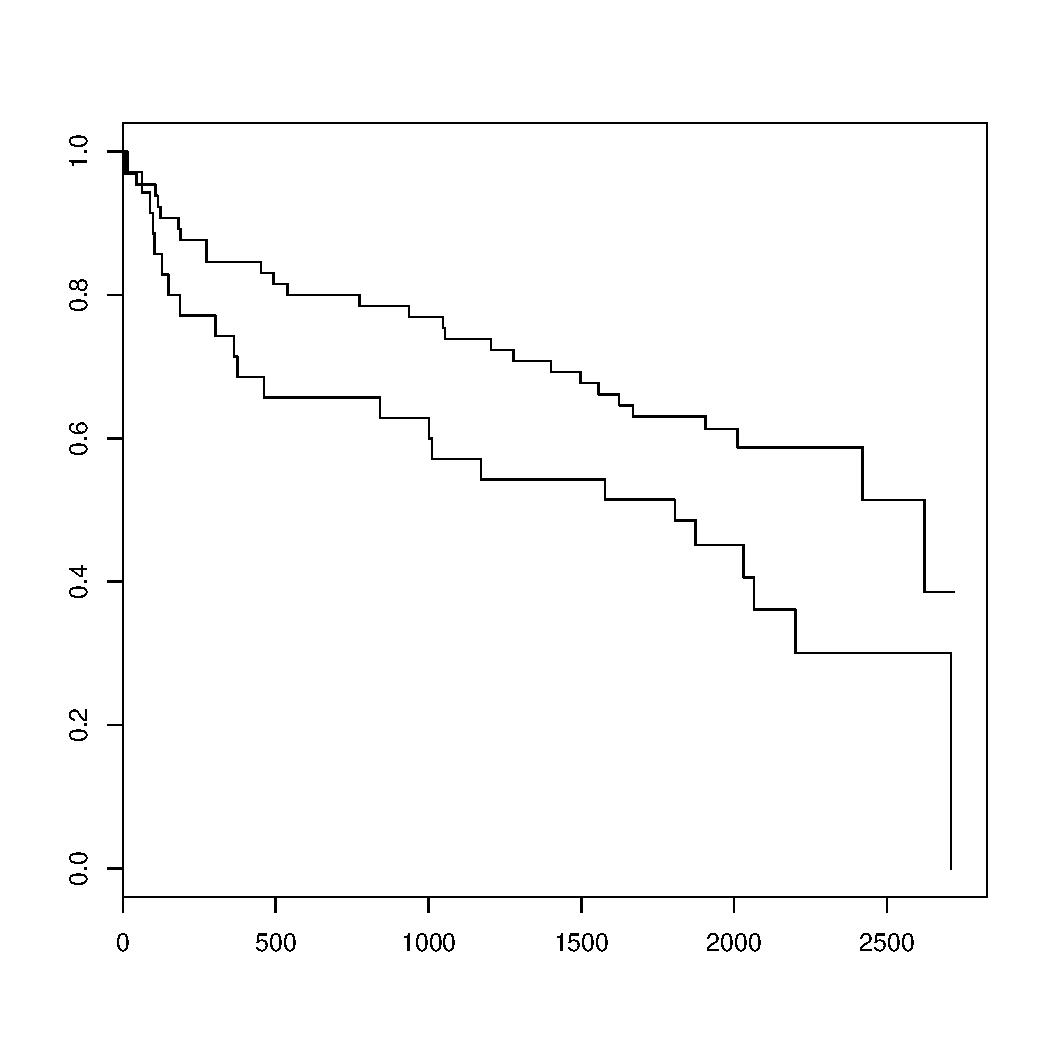
\includegraphics[scale = .26]{km-gender1}\hspace{.2cm}
    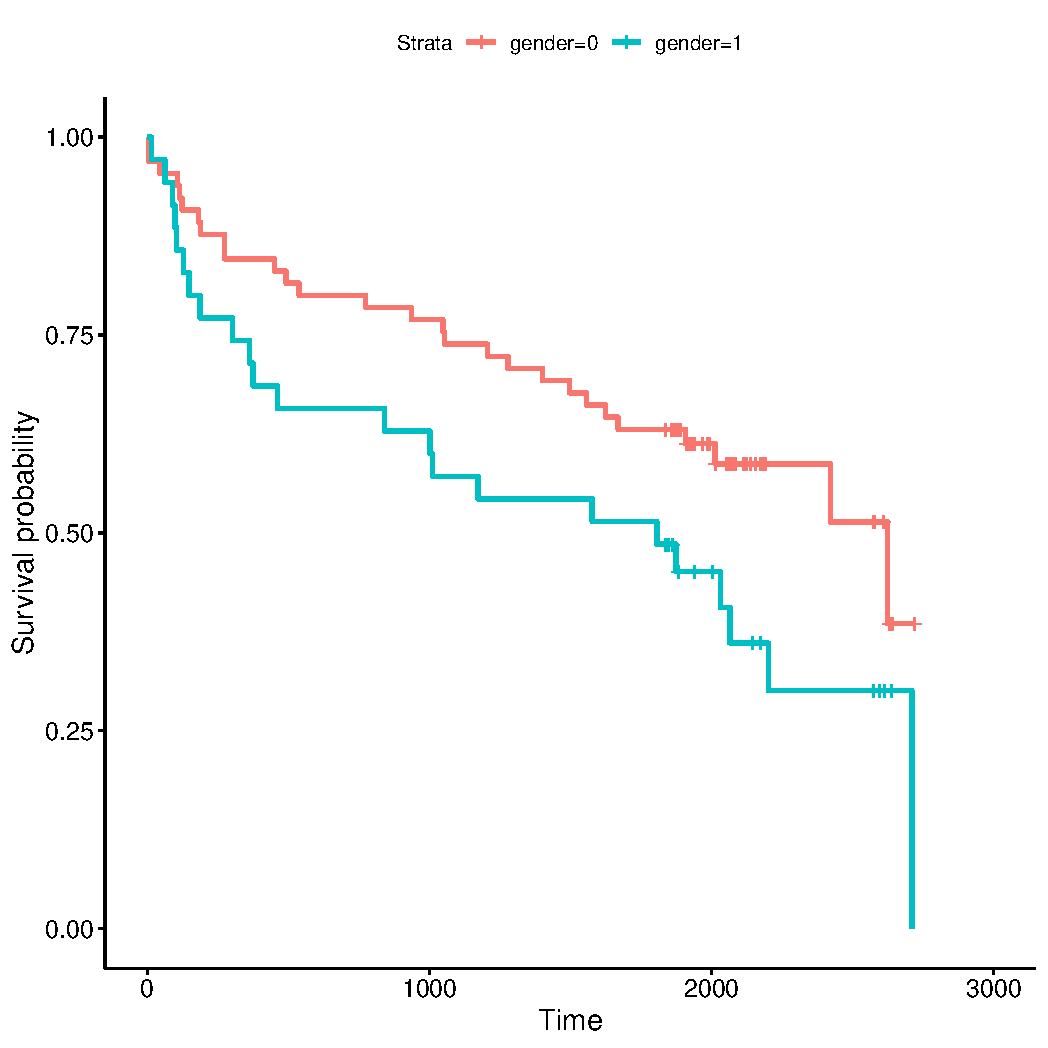
\includegraphics[scale = .26]{km-gender2}
  \end{center}
\end{frame}

\begin{frame}
  \frametitle{Comparison of survival functions}
  \begin{itemize}
  \item In the \code{whas100} study, 
    the survival function for female patients (\code{gender = 0}) is always greater than 
    that for male patients.
  \item Two explanations for the observed difference:
    \begin{itemize}
    \item A real difference between the survival times of the two groups.
    \item The difference has been observed is the result of chance variation. 
    \end{itemize}
  \item Procedures such as the \empr{hypothesis test} is needed to distinguish 
    the two possible explanations. 
  \end{itemize}
\end{frame}

\begin{frame}
  \frametitle{Hypothesis testing}
  \begin{itemize}
  \item As the hypothesis tests commonly encountered, 
    the testing procedure here consists of the following major steps:
    \begin{enumerate}
    \item State the \empr{null hypothesis} and the \empr{alternative hypothesis}. 
    \item Formulate a \empr{test statistic} that measures the extent to which 
      the observed data depart from the null hypothesis. 
    \item Calculate the $p$-value; the probability of obtaining a value as extreme 
      or more extreme than the observed value, when the null hypothesis is true. 
    \end{enumerate}
  \end{itemize}
\end{frame}

\begin{frame}
  \frametitle{Hypothesis testing}
  \begin{itemize}
  \item $p$-value can be interpreted as a measure of the strength of evidence 
    against the null hypothesis.
  \item A $p$-value of 0.000 should be interpreted as $p < 0.001$.
  \item A one-sided hypothesis test is only appropriate when there is 
    no interest in departures from the null hypothesis in the opposite direction.
  \item We will look at non-parametric procedures including the log-rank test and the Wilcoxon test.
  \end{itemize}
\end{frame}

\begin{frame}
  \frametitle{The log-rank test}
  \begin{itemize}
  \item If we are willing to assume survival data follow a particular parametric distribution, 
    we can construct a test based on likelihood theory.
  \item We will derive a nonparametric test using a rank-based procedure.
  \item Suppose the population survival curves are $S_1(t)$ and $S_0(t)$.
  \item Ideally, we would like to test $H_o: S_1(t) = S_0(t)$ versus
    $H_a: S_1(t) > S_0(t)$, $S_1(t) < S_0(t)$, or $S_1(t) \ne S_0(t)$.
  \item Unfortunately, this is difficult because $H_a$ can take a wide range of forms.
  \item Instead, it is more feasible to consider the \empr{Lehman alternative}: 
    \begin{equation}
      \label{eq:lrk}
      H_a: S_1(t) = \left[S_0(t)\right]^\theta, \mbox{ for }\theta > 0.
    \end{equation}
  \end{itemize}
\end{frame}

\begin{frame}
  \frametitle{The log-rank test}
  \begin{itemize}
  \item The hypothesis in~\eqref{eq:lrk} can be view in terms of the hazard functions:
    $$H_o: \lambda_1(t) = \lambda_0(t) \mbox{ versus } H_a: \lambda_1(t) = \theta\lambda_0(t).$$
  \item Either way, we could rewrite the hypothesis test as
    $$H_o: \theta = 1 \mbox{ versus } H_a: \theta> 1, \mbox{ or } \theta < 1, \mbox{ or } \theta\ne 1.$$
  \item One can interpret the results solely based on $\theta$ too. 
  \item For example, under $H_a: \theta > 1$, then 
    \begin{itemize}
      \item $S_1(t)$ will be uniformly lower than $S_0(t)$.
      \item $h_1(t)$ will be uniformly higher than $h_0(t)$.
    \end{itemize}
  \end{itemize}
\end{frame}

\begin{frame}
  \frametitle{The log-rank test}
  \begin{itemize}
  \item Following the notations defined previously, 
    we assume
    \begin{itemize} 
    \item the two independent random samples are of size $N_0$ and $N_1$.
    \item $D$ is the total number of events in the combined sample (size $N_0 + N_1$).     
    \item $\{t_{(1)}, \ldots, t_{(D)}\}$ is the ordered event times. 
    \item Let $d_{0i}$ and $d_{1i}$ are the number of events in group 0 and 1, respectively.
    \item Let $n_{0i}$ and $n_{1i}$ are the number of at risk in group 0 and 1, respectively.
    \end{itemize}
  \end{itemize}
\end{frame}

\begin{frame}
  \frametitle{The log-rank test}
  \begin{itemize}
  \item For the $i$th event time, we construct the following two-by-two table:
  \end{itemize}
  \renewcommand{\arraystretch}{1.3}
  \begin{center}
    \begin{tabular}{cccc}
      &Group 1&Group 0& Total\\
      \cline{2-3}
      Failure &\multicolumn{1}{|c|}{$d_{1i}$}&\multicolumn{1}{|c|}{$d_{0i}$}&$d_i$\\
      \cline{2-3}
      Non-failure &\multicolumn{1}{|c|}{$n_{1i}-d_{1i}$}&\multicolumn{1}{|c|}{$n_{0i}-d_{0i}$}&$n_i-d_i$\\
      \cline{2-3}
      At risk & $n_{1i}$ &  $n_{0i}$ & $n_i$\\
    \end{tabular}
  \end{center}
  \begin{itemize}
  \item Suppose the numbers of failures in two groups are independent, 
    holding the margins fixed, % ($d_i$, $n_i-d_I$, $n_{1i}$ and $n_{0i}$) fixed, 
    then the distribution of $d_{1i}$ (or $d_{0i}$) follows a \emph{hypergeometric distribution}. 
  \item This gives
    \begin{equation*}
      \E(d_{1i}) = \frac{n_{1i} \cdot d_i}{n_i}, \mbox{ and } \Var(d_{1i}) = \frac{n_{1i}\cdot n_{0i}\cdot d_i\cdot(n_i - d_i)}{n_i^2\cdot(n_i-1)}.
    \end{equation*}
  \end{itemize}
\end{frame}

\begin{frame}
  \frametitle{The log-rank test}
  \begin{itemize}
  \item Using the idea from the $\chi^2$ tests, the test statistic has the form 
    \begin{equation}
      \label{eq:chi}
      Q = \frac{\left[\sum_{i = 1}^D\omega_i\{d_{1i} - \E(d_{1i})\}\right]^2}{\sum_{i = 1}^D\omega_i^2\Var(d_{1i})},
  \end{equation}
  where $\omega_i$ is a possibly data-dependent weight.
\item When there is no tied failure times, $\Var(d_{1i}) = \frac{n_{1i}\cdot n_{0i}}{n_i^2}$.
\item Under the null, $Q$ follows the $\chi^2$ distribution with one degree of freedom. 
  \item The log-rank test sets $\omega_i = 1$ \citep{peto1972asymptotically}.
  \end{itemize}
\end{frame}    

\begin{frame}
  \frametitle{The log-rank test}
  \begin{itemize}
  \item Different selections of $\omega_i$ were studied. 
  \item Most common expression has the form of
    $$ \omega_i = \left\{\hat{S}(t_{(i)})\right\}^\rho, \mbox{ for }\rho \in [0, 1],$$
    where $\hat{S}(t)$ is the survival estimator from the combined sample, ignoring group.
  \item This is called the Fleming-Harrington $G(\rho)$ test \citep[e.g.][]{cox1984analysis, harrington1982class}.
    \begin{itemize}
    \item $\rho = 0$ gives the log-rank test
    \item $\rho = 1$ gives the Wilcoxon test.
    \item $\rho = 0.5$ gives the \citet{tarone1977distribution} test.
    \end{itemize}
  \end{itemize}
\end{frame}

\begin{frame}[fragile]
  \frametitle{The log-rank test}
  \begin{itemize}
  \item The $G(\rho)$ test is implemented in \code{survdiff} of the \pkg{survival} package
\begin{knitrout}\scriptsize
\definecolor{shadecolor}{rgb}{0.969, 0.969, 0.969}\color{fgcolor}\begin{kframe}
\begin{alltt}
\hlstd{> }\hlkwd{args}\hlstd{(survdiff)}
\end{alltt}
\begin{verbatim}
function (formula, data, subset, na.action, rho = 0) 
NULL
\end{verbatim}
\begin{alltt}
\hlstd{> }\hlkwd{survdiff}\hlstd{(}\hlkwd{Surv}\hlstd{(lenfol, fstat)} \hlopt{~} \hlstd{gender,} \hlkwc{data} \hlstd{= whas100)}
\end{alltt}
\begin{verbatim}
Call:
survdiff(formula = Surv(lenfol, fstat) ~ gender, data = whas100)

          N Observed Expected (O-E)^2/E (O-E)^2/V
gender=0 65       28     34.6      1.27      3.97
gender=1 35       23     16.4      2.68      3.97

 Chisq= 4  on 1 degrees of freedom, p= 0.05 
\end{verbatim}
\end{kframe}
\end{knitrout}
  \item The log-rank test shows \code{gender} is marginally significant at $\alpha = 0.05$.
  \end{itemize}
\end{frame}


\begin{frame}
  \frametitle{The log-rank test}
  \begin{itemize}
  \item Varying $\rho$ shows similar results here.
  \item In general, when the tests give different results, then more than one result should be reported.
  \item It is important to also consult the plot to ascertain the directional effect of stratification or treatment.
  \end{itemize}
\end{frame}


\begin{frame}
  \frametitle{The log-rank test}
  \begin{itemize}
  \item As in the Pearson's $\chi^2$ test, a continuity correction could be considered when sample sizes are too small: 
    \begin{equation*}
      Q^*= \frac{\left[\sum_{i = 1}^D\omega_i\{|d_{1i} - \E(d_{1i})| - 0.5\}\right]^2}{\sum_{i = 1}^D\omega_i^2\Var(d_{1i})}.
      \end{equation*}
  \end{itemize}
\end{frame}


\begin{frame}
  \frametitle{The log-rank test}
  \begin{itemize}
  \item A problem can occur if the estimated survival (hazard) functions cross one another. 
  \item This is similar to the proportional hazard assumption in the Cox models.
  \item In \code{whas100} data, the two survival curves (by gener) crossed one another at early $t$, 
    despite being so different in large $t$.
  \item \citet{fleming1987supremum} proposed supremum versions of the log-rank tests, but have not been implemented in any software packages.
  \end{itemize}
\end{frame}


\begin{frame}
  \frametitle{The log-rank test}
  \begin{itemize}
  \item The tests discussed here can be extended to comparison more than two survival functions simultaneously.
  \item $K$-by-$K$ tables instead of two-by-two tables at each event time.
  \item When there are many groups to compare, it might be more convenient to consider regression models.
  \end{itemize}
\end{frame}


\section{Reference}
\begin{frame}[shrink = 25]
\frametitle{Reference}
\begin{center}
\scriptsize
\bibliographystyle{biom}
\bibliography{stat6390}
\end{center}
\end{frame}

\end{document}


